\documentclass[twoside]{book}

% Packages required by doxygen
\usepackage{calc}
\usepackage{doxygen}
\usepackage{graphicx}
\usepackage[utf8]{inputenc}
\usepackage{makeidx}
\usepackage{multicol}
\usepackage{multirow}
\usepackage{textcomp}
\usepackage[table]{xcolor}

% Font selection
\usepackage[T1]{fontenc}
\usepackage{mathptmx}
\usepackage[scaled=.90]{helvet}
\usepackage{courier}
\usepackage{amssymb}
\usepackage{sectsty}
\renewcommand{\familydefault}{\sfdefault}
\allsectionsfont{%
  \fontseries{bc}\selectfont%
  \color{darkgray}%
}
\renewcommand{\DoxyLabelFont}{%
  \fontseries{bc}\selectfont%
  \color{darkgray}%
}

% Page & text layout
\usepackage{geometry}
\geometry{%
  a4paper,%
  top=2.5cm,%
  bottom=2.5cm,%
  left=2.5cm,%
  right=2.5cm%
}
\tolerance=750
\hfuzz=15pt
\hbadness=750
\setlength{\emergencystretch}{15pt}
\setlength{\parindent}{0cm}
\setlength{\parskip}{0.2cm}
\makeatletter
\renewcommand{\paragraph}{%
  \@startsection{paragraph}{4}{0ex}{-1.0ex}{1.0ex}{%
    \normalfont\normalsize\bfseries\SS@parafont%
  }%
}
\renewcommand{\subparagraph}{%
  \@startsection{subparagraph}{5}{0ex}{-1.0ex}{1.0ex}{%
    \normalfont\normalsize\bfseries\SS@subparafont%
  }%
}
\makeatother

% Headers & footers
\usepackage{fancyhdr}
\pagestyle{fancyplain}
\fancyhead[LE]{\fancyplain{}{\bfseries\thepage}}
\fancyhead[CE]{\fancyplain{}{}}
\fancyhead[RE]{\fancyplain{}{\bfseries\leftmark}}
\fancyhead[LO]{\fancyplain{}{\bfseries\rightmark}}
\fancyhead[CO]{\fancyplain{}{}}
\fancyhead[RO]{\fancyplain{}{\bfseries\thepage}}
\fancyfoot[LE]{\fancyplain{}{}}
\fancyfoot[CE]{\fancyplain{}{}}
\fancyfoot[RE]{\fancyplain{}{\bfseries\scriptsize Generated on Thu Jan 9 2014 03\-:06\-:05 for Thenaterweb by Doxygen }}
\fancyfoot[LO]{\fancyplain{}{\bfseries\scriptsize Generated on Thu Jan 9 2014 03\-:06\-:05 for Thenaterweb by Doxygen }}
\fancyfoot[CO]{\fancyplain{}{}}
\fancyfoot[RO]{\fancyplain{}{}}
\renewcommand{\footrulewidth}{0.4pt}
\renewcommand{\chaptermark}[1]{%
  \markboth{#1}{}%
}
\renewcommand{\sectionmark}[1]{%
  \markright{\thesection\ #1}%
}

% Indices & bibliography
\usepackage{natbib}
\usepackage[titles]{tocloft}
\setcounter{tocdepth}{3}
\setcounter{secnumdepth}{5}
\makeindex

% Hyperlinks (required, but should be loaded last)
\usepackage{ifpdf}
\ifpdf
  \usepackage[pdftex,pagebackref=true]{hyperref}
\else
  \usepackage[ps2pdf,pagebackref=true]{hyperref}
\fi
\hypersetup{%
  colorlinks=true,%
  linkcolor=blue,%
  citecolor=blue,%
  unicode%
}

% Custom commands
\newcommand{\clearemptydoublepage}{%
  \newpage{\pagestyle{empty}\cleardoublepage}%
}


%===== C O N T E N T S =====

\begin{document}

% Titlepage & ToC
\hypersetup{pageanchor=false}
\pagenumbering{roman}
\begin{titlepage}
\vspace*{7cm}
\begin{center}%
{\Large Thenaterweb }\\
\vspace*{1cm}
{\large Generated by Doxygen 1.8.6}\\
\vspace*{0.5cm}
{\small Thu Jan 9 2014 03:06:05}\\
\end{center}
\end{titlepage}
\clearemptydoublepage
\tableofcontents
\clearemptydoublepage
\pagenumbering{arabic}
\hypersetup{pageanchor=true}

%--- Begin generated contents ---
\chapter{Namespace Index}
\section{Namespace List}
Here is a list of all documented namespaces with brief descriptions\-:\begin{DoxyCompactList}
\item\contentsline{section}{\hyperlink{namespaceDatabaseAccess}{Database\-Access} }{\pageref{namespaceDatabaseAccess}}{}
\end{DoxyCompactList}

\chapter{Hierarchical Index}
\section{Class Hierarchy}
This inheritance list is sorted roughly, but not completely, alphabetically\-:\begin{DoxyCompactList}
\item \contentsline{section}{config}{\pageref{classconfig}}{}
\item \contentsline{section}{Controller\-Base}{\pageref{classControllerBase}}{}
\begin{DoxyCompactList}
\item \contentsline{section}{auth}{\pageref{classauth}}{}
\item \contentsline{section}{feeds}{\pageref{classfeeds}}{}
\item \contentsline{section}{sitemaps}{\pageref{classsitemaps}}{}
\end{DoxyCompactList}
\item \contentsline{section}{Data\-Access\-Layer}{\pageref{classDataAccessLayer}}{}
\item \contentsline{section}{Database}{\pageref{classDatabase}}{}
\item \contentsline{section}{data\-Monger}{\pageref{classdataMonger}}{}
\begin{DoxyCompactList}
\item \contentsline{section}{article}{\pageref{classarticle}}{}
\begin{DoxyCompactList}
\item \contentsline{section}{mapped\-Article}{\pageref{classmappedArticle}}{}
\item \contentsline{section}{std\-Class\-Article}{\pageref{classstdClassArticle}}{}
\end{DoxyCompactList}
\item \contentsline{section}{feed}{\pageref{classfeed}}{}
\item \contentsline{section}{url}{\pageref{classurl}}{}
\end{DoxyCompactList}
\item \contentsline{section}{engine}{\pageref{classengine}}{}
\item \contentsline{section}{Error\-Stack}{\pageref{classErrorStack}}{}
\item \contentsline{section}{Extension}{\pageref{interfaceExtension}}{}
\item \contentsline{section}{File}{\pageref{classFile}}{}
\item \contentsline{section}{lock}{\pageref{classlock}}{}
\item \contentsline{section}{Model}{\pageref{classModel}}{}
\item model\-Base\begin{DoxyCompactList}
\item \contentsline{section}{nw\-Group}{\pageref{classnwGroup}}{}
\item \contentsline{section}{nw\-User}{\pageref{classnwUser}}{}
\end{DoxyCompactList}
\item \contentsline{section}{Model\-Base}{\pageref{classModelBase}}{}
\item \contentsline{section}{redirect}{\pageref{classredirect}}{}
\begin{DoxyCompactList}
\item \contentsline{section}{cond\-Redirect}{\pageref{classcondRedirect}}{}
\end{DoxyCompactList}
\item \contentsline{section}{request}{\pageref{classrequest}}{}
\item \contentsline{section}{Session\-Mgr}{\pageref{classSessionMgr}}{}
\item \contentsline{section}{url\-Handler}{\pageref{classurlHandler}}{}
\item \contentsline{section}{urlset}{\pageref{classurlset}}{}
\end{DoxyCompactList}

\chapter{Class Index}
\section{Class List}
Here are the classes, structs, unions and interfaces with brief descriptions\-:\begin{DoxyCompactList}
\item\contentsline{section}{\hyperlink{classarticle}{article} }{\pageref{classarticle}}{}
\item\contentsline{section}{\hyperlink{classauth}{auth} }{\pageref{classauth}}{}
\item\contentsline{section}{\hyperlink{classcondRedirect}{cond\-Redirect} }{\pageref{classcondRedirect}}{}
\item\contentsline{section}{\hyperlink{classconfig}{config} }{\pageref{classconfig}}{}
\item\contentsline{section}{\hyperlink{classcontrollerBase}{controller\-Base} }{\pageref{classcontrollerBase}}{}
\item\contentsline{section}{\hyperlink{classDataAccessLayer}{Data\-Access\-Layer} }{\pageref{classDataAccessLayer}}{}
\item\contentsline{section}{\hyperlink{classDatabase}{Database} }{\pageref{classDatabase}}{}
\item\contentsline{section}{\hyperlink{classdataMonger}{data\-Monger} }{\pageref{classdataMonger}}{}
\item\contentsline{section}{\hyperlink{classdirectoryIndex}{directory\-Index} }{\pageref{classdirectoryIndex}}{}
\item\contentsline{section}{\hyperlink{classengine}{engine} }{\pageref{classengine}}{}
\item\contentsline{section}{\hyperlink{classErrorStack}{Error\-Stack} }{\pageref{classErrorStack}}{}
\item\contentsline{section}{\hyperlink{interfaceExtension}{Extension} }{\pageref{interfaceExtension}}{}
\item\contentsline{section}{\hyperlink{classfeed}{feed} }{\pageref{classfeed}}{}
\item\contentsline{section}{\hyperlink{classfeeds}{feeds} }{\pageref{classfeeds}}{}
\item\contentsline{section}{\hyperlink{classFile}{File} }{\pageref{classFile}}{}
\item\contentsline{section}{\hyperlink{classjsonMaker}{json\-Maker} }{\pageref{classjsonMaker}}{}
\item\contentsline{section}{\hyperlink{classlock}{lock} }{\pageref{classlock}}{}
\item\contentsline{section}{\hyperlink{classmappedArticle}{mapped\-Article} }{\pageref{classmappedArticle}}{}
\item\contentsline{section}{\hyperlink{classModel}{Model} }{\pageref{classModel}}{}
\item\contentsline{section}{\hyperlink{classModelBase}{Model\-Base} }{\pageref{classModelBase}}{}
\item\contentsline{section}{\hyperlink{classnwGroup}{nw\-Group} }{\pageref{classnwGroup}}{}
\item\contentsline{section}{\hyperlink{classnwUser}{nw\-User} }{\pageref{classnwUser}}{}
\item\contentsline{section}{\hyperlink{classredirect}{redirect} }{\pageref{classredirect}}{}
\item\contentsline{section}{\hyperlink{classrequest}{request} }{\pageref{classrequest}}{}
\item\contentsline{section}{\hyperlink{classSessionMgr}{Session\-Mgr} }{\pageref{classSessionMgr}}{}
\item\contentsline{section}{\hyperlink{classsitemaps}{sitemaps} }{\pageref{classsitemaps}}{}
\item\contentsline{section}{\hyperlink{classstdClassArticle}{std\-Class\-Article} }{\pageref{classstdClassArticle}}{}
\item\contentsline{section}{\hyperlink{classurl}{url} }{\pageref{classurl}}{}
\item\contentsline{section}{\hyperlink{classurlHandler}{url\-Handler} }{\pageref{classurlHandler}}{}
\item\contentsline{section}{\hyperlink{classurlset}{urlset} }{\pageref{classurlset}}{}
\end{DoxyCompactList}

\chapter{Namespace Documentation}
\hypertarget{namespaceDatabaseAccess}{\section{Database\-Access Namespace Reference}
\label{namespaceDatabaseAccess}\index{Database\-Access@{Database\-Access}}
}


\subsection{Detailed Description}
Handles all access to data via a database. This file contains classes and functions that interact with the database and database library directly.

Contains the main \hyperlink{classModel}{Model} class which holds utilities for managing model field types.

Contains the base model class that all database-\/using models of applications need to inherit from. 
\chapter{Class Documentation}
\hypertarget{classarticle}{\section{article Class Reference}
\label{classarticle}\index{article@{article}}
}
Inheritance diagram for article\-:\begin{figure}[H]
\begin{center}
\leavevmode
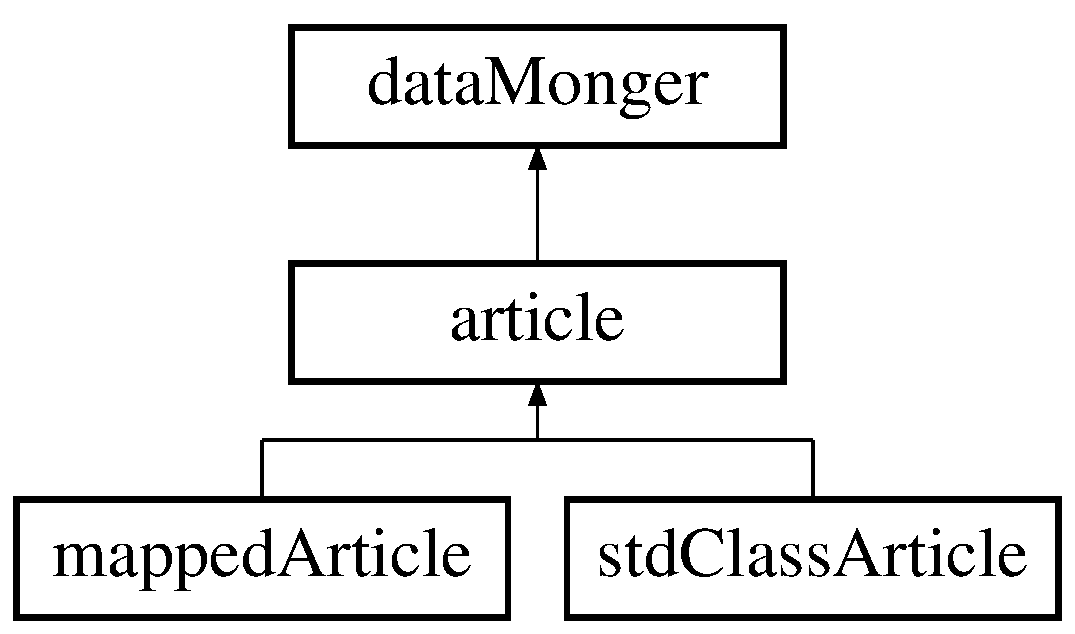
\includegraphics[height=3.000000cm]{classarticle}
\end{center}
\end{figure}
\subsection*{Public Member Functions}
\begin{DoxyCompactItemize}
\item 
\hyperlink{classarticle_abc0c9463fc62baf5b4ef25b8ce546719}{\-\_\-\-\_\-construct} (\$nodefile, \$bloguri, \$article\-Uri=\char`\"{}\char`\"{})
\item 
\hyperlink{classarticle_a388fbd65b6ac1ab943b57284ce69eb56}{output} (\$type)
\item 
\hypertarget{classarticle_acfe6274b03d0051798d935e45d054195}{{\bfseries \-\_\-\-\_\-get} (\$field)}\label{classarticle_acfe6274b03d0051798d935e45d054195}

\item 
\hypertarget{classarticle_a93fcc436140d32b39762d95475474fb3}{{\bfseries get\-Type} ()}\label{classarticle_a93fcc436140d32b39762d95475474fb3}

\item 
\hypertarget{classarticle_afdda7e69ce8567ac2be12214fec5a852}{{\bfseries to\-Html} ()}\label{classarticle_afdda7e69ce8567ac2be12214fec5a852}

\item 
\hypertarget{classarticle_a2a51edc07f4e8ca22aeec3b997a8dc56}{{\bfseries get\-File} ()}\label{classarticle_a2a51edc07f4e8ca22aeec3b997a8dc56}

\item 
\hyperlink{classarticle_a07b78b42ec5aa8cc3423d758038c69fc}{get\-Meta} ()
\item 
\hypertarget{classarticle_a30c5793bc25061365c8b8a79103012be}{{\bfseries is\-Php} ()}\label{classarticle_a30c5793bc25061365c8b8a79103012be}

\item 
\hyperlink{classarticle_a0fdbe317408cbc7eed6fdbac441bb700}{list\-\_\-item\-\_\-output} ()
\end{DoxyCompactItemize}
\subsection*{Protected Attributes}
\begin{DoxyCompactItemize}
\item 
\hypertarget{classarticle_abe7cedd17e5d9f8b2382f523595be405}{{\bfseries \$use\-Post\-Format}}\label{classarticle_abe7cedd17e5d9f8b2382f523595be405}

\end{DoxyCompactItemize}


\subsection{Detailed Description}
Provides a consistent interface for accessing posts or articles with multiple methods of displaying and managing the contained data.

\begin{DoxyAuthor}{Author}
Nate Levesque \href{mailto:public@thenaterhood.com}{\tt public@thenaterhood.\-com} Includes the inherited \hyperlink{classdataMonger}{data\-Monger} class Contains everything to do with retrieving and outputting posts in multiple forms. Is capable of retrieving posts stored in .json format (preferred when available) as well as plaintext (file syntax described below in constructor).
\end{DoxyAuthor}
Contains functions to output the post data in html format for displaying to a page, and atom format for use in generating an atom feed. 

\subsection{Constructor \& Destructor Documentation}
\hypertarget{classarticle_abc0c9463fc62baf5b4ef25b8ce546719}{\index{article@{article}!\-\_\-\-\_\-construct@{\-\_\-\-\_\-construct}}
\index{\-\_\-\-\_\-construct@{\-\_\-\-\_\-construct}!article@{article}}
\subsubsection[{\-\_\-\-\_\-construct}]{\setlength{\rightskip}{0pt plus 5cm}article\-::\-\_\-\-\_\-construct (
\begin{DoxyParamCaption}
\item[{}]{\$nodefile, }
\item[{}]{\$bloguri, }
\item[{}]{\$article\-Uri = {\ttfamily \char`\"{}\char`\"{}}}
\end{DoxyParamCaption}
)}}\label{classarticle_abc0c9463fc62baf5b4ef25b8ce546719}
Reads and parses a post file and creates an instance of the class with the post data. Capable of managing posts in json and plaintext, but prefers json if a json file exists for the requested post.


\begin{DoxyParams}{Parameters}
{\em nodefile} & (string) -\/ a yyyy.\-mm.\-dd string of a nodefile \\
\hline
\end{DoxyParams}


\subsection{Member Function Documentation}
\hypertarget{classarticle_a07b78b42ec5aa8cc3423d758038c69fc}{\index{article@{article}!get\-Meta@{get\-Meta}}
\index{get\-Meta@{get\-Meta}!article@{article}}
\subsubsection[{get\-Meta}]{\setlength{\rightskip}{0pt plus 5cm}article\-::get\-Meta (
\begin{DoxyParamCaption}
{}
\end{DoxyParamCaption}
)}}\label{classarticle_a07b78b42ec5aa8cc3423d758038c69fc}
Returns the article metadata -\/ tags, title, link, date, and author as an associative array. \begin{DoxyReturn}{Returns}
\$meta -\/ the metadata array 
\end{DoxyReturn}
\hypertarget{classarticle_a0fdbe317408cbc7eed6fdbac441bb700}{\index{article@{article}!list\-\_\-item\-\_\-output@{list\-\_\-item\-\_\-output}}
\index{list\-\_\-item\-\_\-output@{list\-\_\-item\-\_\-output}!article@{article}}
\subsubsection[{list\-\_\-item\-\_\-output}]{\setlength{\rightskip}{0pt plus 5cm}article\-::list\-\_\-item\-\_\-output (
\begin{DoxyParamCaption}
{}
\end{DoxyParamCaption}
)}}\label{classarticle_a0fdbe317408cbc7eed6fdbac441bb700}
Returns a string containing the post title and tags, suitable for outputting in an atom feed (maybe) or an html list \hypertarget{classarticle_a388fbd65b6ac1ab943b57284ce69eb56}{\index{article@{article}!output@{output}}
\index{output@{output}!article@{article}}
\subsubsection[{output}]{\setlength{\rightskip}{0pt plus 5cm}article\-::output (
\begin{DoxyParamCaption}
\item[{}]{\$type}
\end{DoxyParamCaption}
)}}\label{classarticle_a388fbd65b6ac1ab943b57284ce69eb56}
Returns a representation of the post in the format requested


\begin{DoxyParams}{Parameters}
{\em \$type} & -\/ the type of feed \\
\hline
\end{DoxyParams}


The documentation for this class was generated from the following file\-:\begin{DoxyCompactItemize}
\item 
engine/classes/class\-\_\-article.\-php\end{DoxyCompactItemize}

\hypertarget{classauth}{\section{auth Class Reference}
\label{classauth}\index{auth@{auth}}
}
Inheritance diagram for auth\-:\begin{figure}[H]
\begin{center}
\leavevmode
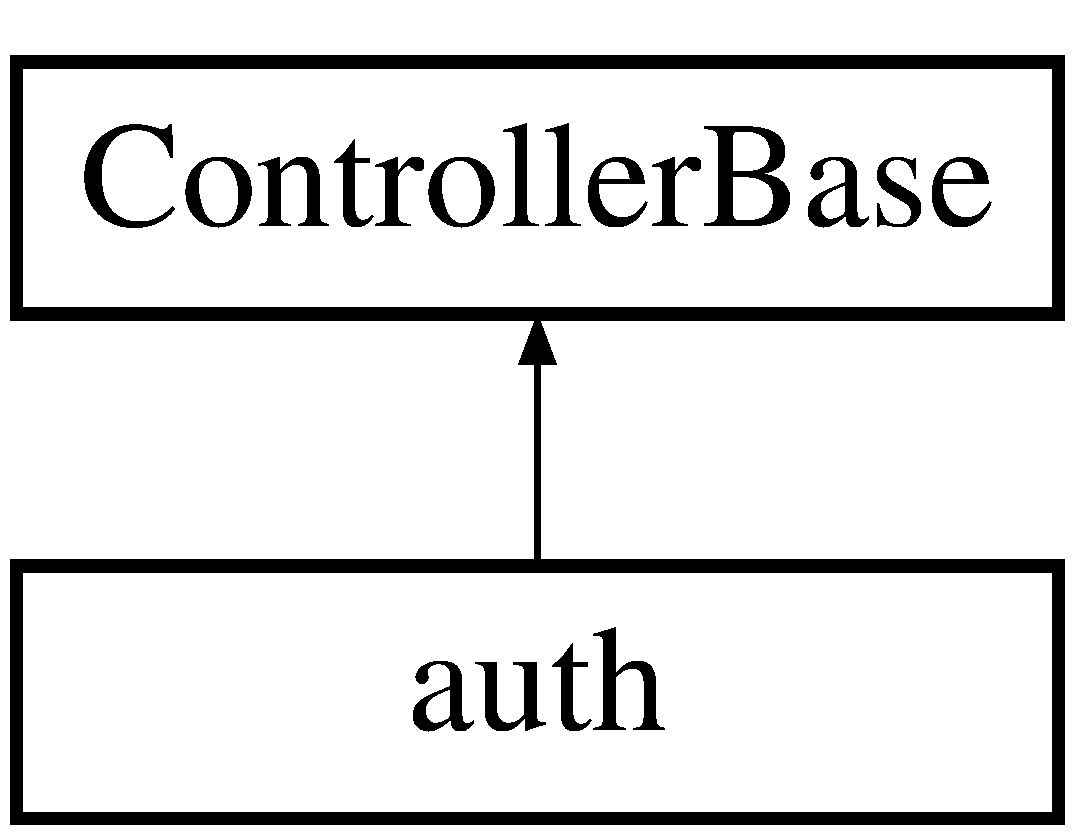
\includegraphics[height=2.000000cm]{classauth}
\end{center}
\end{figure}
\subsection*{Public Member Functions}
\begin{DoxyCompactItemize}
\item 
\hyperlink{classauth_a689697937763dd16e7e859ae430a38d3}{login} ()
\item 
\hyperlink{classauth_ae383d989a03975d0bc61c09a38e0118d}{managegroup} ()
\item 
\hyperlink{classauth_ab982268ed2adefb8cf986947b9751dab}{addgroup} ()
\item 
\hyperlink{classauth_a065eb7c74c5e51991f0d7581029aa14b}{deluser} ()
\item 
\hyperlink{classauth_a94e4cb4b38ca879867f4cd5fdb74a69c}{changeuser} ()
\item 
\hyperlink{classauth_a4d44da80906dcf985cd50ce4b154e86e}{adduser} ()
\item 
\hyperlink{classauth_ab0dc3734583e1b7fe4a7b2f76e3b117a}{manage} ()
\item 
\hyperlink{classauth_a1eae8dfe52748742162182fe1b19255e}{check\-\_\-login} (\$user, \$plainpasswd)
\item 
\hypertarget{classauth_acf39697e476e9213d8c5ed9e98f45108}{{\bfseries logout} ()}\label{classauth_acf39697e476e9213d8c5ed9e98f45108}

\end{DoxyCompactItemize}
\subsection*{Additional Inherited Members}


\subsection{Member Function Documentation}
\hypertarget{classauth_ab982268ed2adefb8cf986947b9751dab}{\index{auth@{auth}!addgroup@{addgroup}}
\index{addgroup@{addgroup}!auth@{auth}}
\subsubsection[{addgroup}]{\setlength{\rightskip}{0pt plus 5cm}auth\-::addgroup (
\begin{DoxyParamCaption}
{}
\end{DoxyParamCaption}
)}}\label{classauth_ab982268ed2adefb8cf986947b9751dab}
Renders the add group page where a group can be added. \hypertarget{classauth_a4d44da80906dcf985cd50ce4b154e86e}{\index{auth@{auth}!adduser@{adduser}}
\index{adduser@{adduser}!auth@{auth}}
\subsubsection[{adduser}]{\setlength{\rightskip}{0pt plus 5cm}auth\-::adduser (
\begin{DoxyParamCaption}
{}
\end{DoxyParamCaption}
)}}\label{classauth_a4d44da80906dcf985cd50ce4b154e86e}
Adds a new user to the system \hypertarget{classauth_a94e4cb4b38ca879867f4cd5fdb74a69c}{\index{auth@{auth}!changeuser@{changeuser}}
\index{changeuser@{changeuser}!auth@{auth}}
\subsubsection[{changeuser}]{\setlength{\rightskip}{0pt plus 5cm}auth\-::changeuser (
\begin{DoxyParamCaption}
{}
\end{DoxyParamCaption}
)}}\label{classauth_a94e4cb4b38ca879867f4cd5fdb74a69c}
Updates a user's information and groups \hypertarget{classauth_a1eae8dfe52748742162182fe1b19255e}{\index{auth@{auth}!check\-\_\-login@{check\-\_\-login}}
\index{check\-\_\-login@{check\-\_\-login}!auth@{auth}}
\subsubsection[{check\-\_\-login}]{\setlength{\rightskip}{0pt plus 5cm}auth\-::check\-\_\-login (
\begin{DoxyParamCaption}
\item[{}]{\$user, }
\item[{}]{\$plainpasswd}
\end{DoxyParamCaption}
)}}\label{classauth_a1eae8dfe52748742162182fe1b19255e}
Checks a user's credentials with the database or a .htaccess file depending on the setup. \hypertarget{classauth_a065eb7c74c5e51991f0d7581029aa14b}{\index{auth@{auth}!deluser@{deluser}}
\index{deluser@{deluser}!auth@{auth}}
\subsubsection[{deluser}]{\setlength{\rightskip}{0pt plus 5cm}auth\-::deluser (
\begin{DoxyParamCaption}
{}
\end{DoxyParamCaption}
)}}\label{classauth_a065eb7c74c5e51991f0d7581029aa14b}
Deletes a user from the database along with their group associations. \hypertarget{classauth_a689697937763dd16e7e859ae430a38d3}{\index{auth@{auth}!login@{login}}
\index{login@{login}!auth@{auth}}
\subsubsection[{login}]{\setlength{\rightskip}{0pt plus 5cm}auth\-::login (
\begin{DoxyParamCaption}
{}
\end{DoxyParamCaption}
)}}\label{classauth_a689697937763dd16e7e859ae430a38d3}
Logs a user in after validating their credentials, or redirects back to the login page. \hypertarget{classauth_ab0dc3734583e1b7fe4a7b2f76e3b117a}{\index{auth@{auth}!manage@{manage}}
\index{manage@{manage}!auth@{auth}}
\subsubsection[{manage}]{\setlength{\rightskip}{0pt plus 5cm}auth\-::manage (
\begin{DoxyParamCaption}
{}
\end{DoxyParamCaption}
)}}\label{classauth_ab0dc3734583e1b7fe4a7b2f76e3b117a}
Shows the main user management page \hypertarget{classauth_ae383d989a03975d0bc61c09a38e0118d}{\index{auth@{auth}!managegroup@{managegroup}}
\index{managegroup@{managegroup}!auth@{auth}}
\subsubsection[{managegroup}]{\setlength{\rightskip}{0pt plus 5cm}auth\-::managegroup (
\begin{DoxyParamCaption}
{}
\end{DoxyParamCaption}
)}}\label{classauth_ae383d989a03975d0bc61c09a38e0118d}
Renders the group management page where groups can be added. 

The documentation for this class was generated from the following file\-:\begin{DoxyCompactItemize}
\item 
engine/lib/builtins/auth/main.\-php\end{DoxyCompactItemize}

\hypertarget{classcondRedirect}{\section{cond\-Redirect Class Reference}
\label{classcondRedirect}\index{cond\-Redirect@{cond\-Redirect}}
}
Inheritance diagram for cond\-Redirect\-:\begin{figure}[H]
\begin{center}
\leavevmode
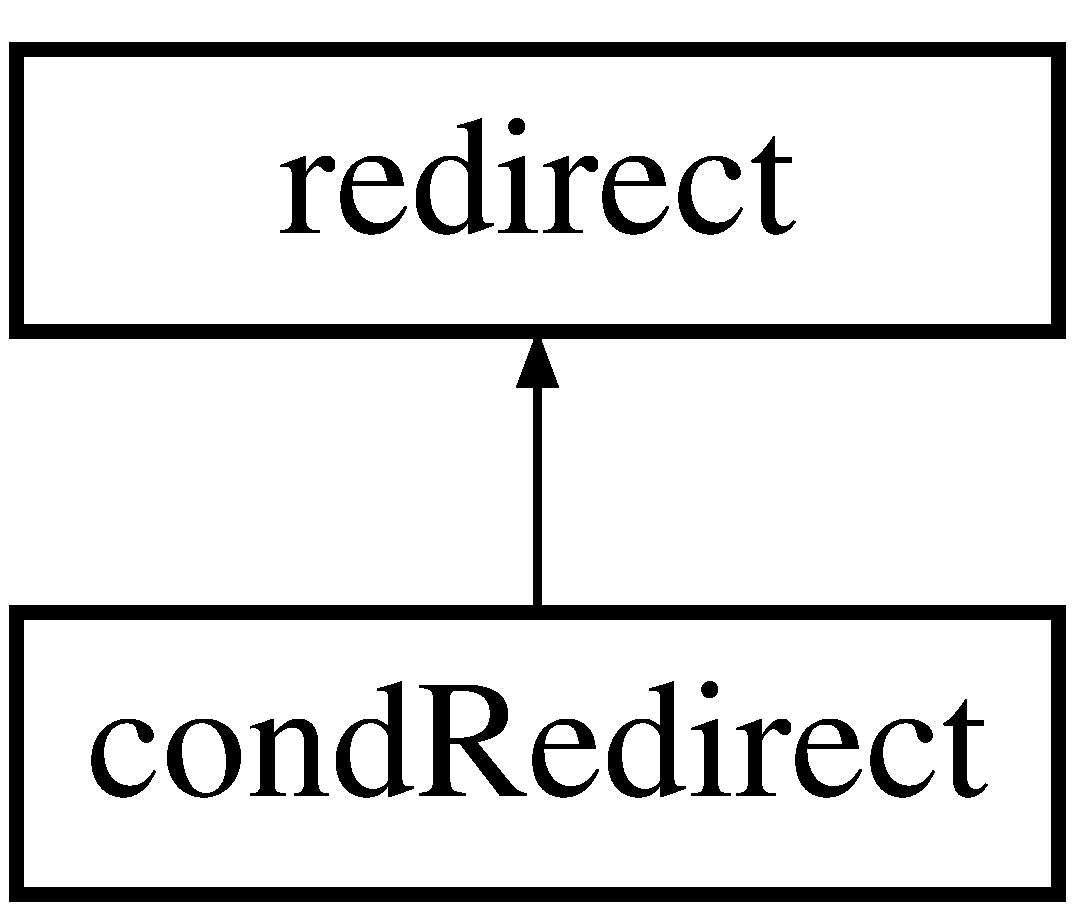
\includegraphics[height=2.000000cm]{classcondRedirect}
\end{center}
\end{figure}
\subsection*{Public Member Functions}
\begin{DoxyCompactItemize}
\item 
\hyperlink{classcondRedirect_ad18d689973246f0b672e27b969f3ce31}{\-\_\-\-\_\-construct} (\$origin, \$destination, \$uri)
\item 
\hyperlink{classcondRedirect_aeeb36f32e9bf27e34c5806efeb41d35a}{apply} (\$type)
\end{DoxyCompactItemize}
\subsection*{Additional Inherited Members}


\subsection{Detailed Description}
Provides a means of redirecting a page conditionally based on whether the destination is where the user currently is or not. \begin{DoxyAuthor}{Author}
Nate Levesque \href{mailto:public@thenaterhood.com}{\tt public@thenaterhood.\-com} Include the extended redirect class Manages conditionally redirecting pages based on the requested uri and a given uri to redirect from. Checks to see if the uri requested by the user contains the uri to redirect from, and prepares to perform the redirect if so.
\end{DoxyAuthor}
Relies on the redirect class to manage the actual redirecting, this class is primarly an interface to it that deals with the conditional aspect. 

\subsection{Constructor \& Destructor Documentation}
\hypertarget{classcondRedirect_ad18d689973246f0b672e27b969f3ce31}{\index{cond\-Redirect@{cond\-Redirect}!\-\_\-\-\_\-construct@{\-\_\-\-\_\-construct}}
\index{\-\_\-\-\_\-construct@{\-\_\-\-\_\-construct}!condRedirect@{cond\-Redirect}}
\subsubsection[{\-\_\-\-\_\-construct}]{\setlength{\rightskip}{0pt plus 5cm}cond\-Redirect\-::\-\_\-\-\_\-construct (
\begin{DoxyParamCaption}
\item[{}]{\$origin, }
\item[{}]{\$destination, }
\item[{}]{\$uri}
\end{DoxyParamCaption}
)}}\label{classcondRedirect_ad18d689973246f0b672e27b969f3ce31}
Creates an instance of the conditional redirect class and decides whether the redirect will be performed


\begin{DoxyParams}{Parameters}
{\em \$origin} & -\/ a chosen uri to redirect from \\
\hline
{\em \$destination} & -\/ a uri to redirect to \\
\hline
{\em \$uri} & -\/ the uri requested by the user \\
\hline
\end{DoxyParams}


\subsection{Member Function Documentation}
\hypertarget{classcondRedirect_aeeb36f32e9bf27e34c5806efeb41d35a}{\index{cond\-Redirect@{cond\-Redirect}!apply@{apply}}
\index{apply@{apply}!condRedirect@{cond\-Redirect}}
\subsubsection[{apply}]{\setlength{\rightskip}{0pt plus 5cm}cond\-Redirect\-::apply (
\begin{DoxyParamCaption}
\item[{}]{\$type}
\end{DoxyParamCaption}
)}}\label{classcondRedirect_aeeb36f32e9bf27e34c5806efeb41d35a}
Applies the redirect to the page if the redirect should happen


\begin{DoxyParams}{Parameters}
{\em \$type} & -\/ the type of redirect to apply \\
\hline
\end{DoxyParams}


The documentation for this class was generated from the following file\-:\begin{DoxyCompactItemize}
\item 
engine/classes/class\-\_\-cond\-Redirect.\-php\end{DoxyCompactItemize}

\hypertarget{classconfig}{\section{config Class Reference}
\label{classconfig}\index{config@{config}}
}
\subsection*{Public Member Functions}
\begin{DoxyCompactItemize}
\item 
\hyperlink{classconfig_adcf57008d523eae2d6a4ec41340c704c}{\-\_\-\-\_\-construct} ()
\item 
\hyperlink{classconfig_a4d34907fbf3fedfca85fec83cfb894ac}{\-\_\-\-\_\-get} (\$setting)
\end{DoxyCompactItemize}


\subsection{Detailed Description}
Contains configuration settings for the site engine to use as a php class that can be directly accessed.

\begin{DoxyAuthor}{Author}
Nate Levesque \href{mailto:public@thenaterhood.com}{\tt public@thenaterhood.\-com} Language\-: P\-H\-P Filename\-: core\-\_\-config.\-php Defines a class to hold variables for configuration options. All variables are accessible only internally to keep things fairly clean. 
\end{DoxyAuthor}


\subsection{Constructor \& Destructor Documentation}
\hypertarget{classconfig_adcf57008d523eae2d6a4ec41340c704c}{\index{config@{config}!\-\_\-\-\_\-construct@{\-\_\-\-\_\-construct}}
\index{\-\_\-\-\_\-construct@{\-\_\-\-\_\-construct}!config@{config}}
\subsubsection[{\-\_\-\-\_\-construct}]{\setlength{\rightskip}{0pt plus 5cm}config\-::\-\_\-\-\_\-construct (
\begin{DoxyParamCaption}
{}
\end{DoxyParamCaption}
)}}\label{classconfig_adcf57008d523eae2d6a4ec41340c704c}
Sets the configuration options en-\/masse. 

\subsection{Member Function Documentation}
\hypertarget{classconfig_a4d34907fbf3fedfca85fec83cfb894ac}{\index{config@{config}!\-\_\-\-\_\-get@{\-\_\-\-\_\-get}}
\index{\-\_\-\-\_\-get@{\-\_\-\-\_\-get}!config@{config}}
\subsubsection[{\-\_\-\-\_\-get}]{\setlength{\rightskip}{0pt plus 5cm}config\-::\-\_\-\-\_\-get (
\begin{DoxyParamCaption}
\item[{}]{\$setting}
\end{DoxyParamCaption}
)}}\label{classconfig_a4d34907fbf3fedfca85fec83cfb894ac}
Returns the value of the requested config key


\begin{DoxyParams}{Parameters}
{\em \$setting} & -\/ the name of the key\\
\hline
\end{DoxyParams}
\begin{DoxyReturn}{Returns}
-\/ the value the key is associated with 
\end{DoxyReturn}


The documentation for this class was generated from the following file\-:\begin{DoxyCompactItemize}
\item 
settings.\-php\end{DoxyCompactItemize}

\hypertarget{classControllerBase}{\section{Controller\-Base Class Reference}
\label{classControllerBase}\index{Controller\-Base@{Controller\-Base}}
}
Inheritance diagram for Controller\-Base\-:\begin{figure}[H]
\begin{center}
\leavevmode
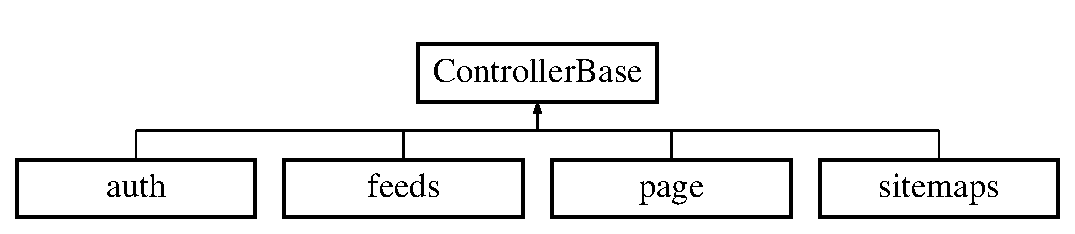
\includegraphics[height=2.000000cm]{classControllerBase}
\end{center}
\end{figure}
\subsection*{Public Member Functions}
\begin{DoxyCompactItemize}
\item 
\hyperlink{classControllerBase_adf22b33f94d79eadbae786f31fdb4b8b}{get\-Configurables} ()
\item 
\hyperlink{classControllerBase_a3de3699fd3f729abfc5fa59decef958f}{read\-Config} (\$path)
\item 
\hyperlink{classControllerBase_ae75dea3157d019d04c663481c60ff201}{save\-Config} (\$path)
\item 
\hyperlink{classControllerBase_afd930559882de5e0d77c5357e07f1af4}{set\-Config} (\$map)
\item 
\hyperlink{classControllerBase_add5cf51bbc1b21b6cea292aed3cb6b29}{\-\_\-\-\_\-get} (\$field)
\item 
\hypertarget{classControllerBase_ad017b0ed4dcdc83cdfa052ceb288366a}{{\bfseries get\-Page\-Data} ()}\label{classControllerBase_ad017b0ed4dcdc83cdfa052ceb288366a}

\item 
\hyperlink{classControllerBase_aae0d40bf6721d92c1a2285ba8edd5ebf}{get\-Page\-List} ()
\item 
\hyperlink{classControllerBase_a0cff8483987ef3926f543d46368a62bf}{get\-Post\-List} ()
\item 
\hypertarget{classControllerBase_a57c3f118de841efa789181fdb1398802}{{\bfseries unauthorized} ()}\label{classControllerBase_a57c3f118de841efa789181fdb1398802}

\end{DoxyCompactItemize}
\subsection*{Protected Attributes}
\begin{DoxyCompactItemize}
\item 
\hypertarget{classControllerBase_a8da9c7c22f36c812ecacc11234337f27}{{\bfseries \$settings}}\label{classControllerBase_a8da9c7c22f36c812ecacc11234337f27}

\item 
\hypertarget{classControllerBase_a7557163c5c72c5e3998e3cb8e71ee5d9}{{\bfseries \$configuration}}\label{classControllerBase_a7557163c5c72c5e3998e3cb8e71ee5d9}

\item 
\hypertarget{classControllerBase_a19f7437237e6e6a3e5bc8493942c3cfc}{{\bfseries \$page\-Data}}\label{classControllerBase_a19f7437237e6e6a3e5bc8493942c3cfc}

\end{DoxyCompactItemize}


\subsection{Member Function Documentation}
\hypertarget{classControllerBase_add5cf51bbc1b21b6cea292aed3cb6b29}{\index{Controller\-Base@{Controller\-Base}!\-\_\-\-\_\-get@{\-\_\-\-\_\-get}}
\index{\-\_\-\-\_\-get@{\-\_\-\-\_\-get}!ControllerBase@{Controller\-Base}}
\subsubsection[{\-\_\-\-\_\-get}]{\setlength{\rightskip}{0pt plus 5cm}Controller\-Base\-::\-\_\-\-\_\-get (
\begin{DoxyParamCaption}
\item[{}]{\$field}
\end{DoxyParamCaption}
)}}\label{classControllerBase_add5cf51bbc1b21b6cea292aed3cb6b29}
Returns requested fields from the settings array.


\begin{DoxyParams}{Parameters}
{\em \$field} & -\/ the name of the item to return \\
\hline
\end{DoxyParams}
\begin{DoxyReturn}{Returns}
the item 
\end{DoxyReturn}
\hypertarget{classControllerBase_adf22b33f94d79eadbae786f31fdb4b8b}{\index{Controller\-Base@{Controller\-Base}!get\-Configurables@{get\-Configurables}}
\index{get\-Configurables@{get\-Configurables}!ControllerBase@{Controller\-Base}}
\subsubsection[{get\-Configurables}]{\setlength{\rightskip}{0pt plus 5cm}Controller\-Base\-::get\-Configurables (
\begin{DoxyParamCaption}
{}
\end{DoxyParamCaption}
)}}\label{classControllerBase_adf22b33f94d79eadbae786f31fdb4b8b}
Returns a map containing all of the controller settings.

\begin{DoxyReturn}{Returns}
a map of the class settings 
\end{DoxyReturn}
\hypertarget{classControllerBase_aae0d40bf6721d92c1a2285ba8edd5ebf}{\index{Controller\-Base@{Controller\-Base}!get\-Page\-List@{get\-Page\-List}}
\index{get\-Page\-List@{get\-Page\-List}!ControllerBase@{Controller\-Base}}
\subsubsection[{get\-Page\-List}]{\setlength{\rightskip}{0pt plus 5cm}Controller\-Base\-::get\-Page\-List (
\begin{DoxyParamCaption}
{}
\end{DoxyParamCaption}
)}}\label{classControllerBase_aae0d40bf6721d92c1a2285ba8edd5ebf}
Returns a list of pages that should be available publicly. Used by the sitemap generation system. \hypertarget{classControllerBase_a0cff8483987ef3926f543d46368a62bf}{\index{Controller\-Base@{Controller\-Base}!get\-Post\-List@{get\-Post\-List}}
\index{get\-Post\-List@{get\-Post\-List}!ControllerBase@{Controller\-Base}}
\subsubsection[{get\-Post\-List}]{\setlength{\rightskip}{0pt plus 5cm}Controller\-Base\-::get\-Post\-List (
\begin{DoxyParamCaption}
{}
\end{DoxyParamCaption}
)}}\label{classControllerBase_a0cff8483987ef3926f543d46368a62bf}
Returns a list of posts (in order) that should be available publicly. Used by the feed generation system. \hypertarget{classControllerBase_a3de3699fd3f729abfc5fa59decef958f}{\index{Controller\-Base@{Controller\-Base}!read\-Config@{read\-Config}}
\index{read\-Config@{read\-Config}!ControllerBase@{Controller\-Base}}
\subsubsection[{read\-Config}]{\setlength{\rightskip}{0pt plus 5cm}Controller\-Base\-::read\-Config (
\begin{DoxyParamCaption}
\item[{}]{\$path}
\end{DoxyParamCaption}
)}}\label{classControllerBase_a3de3699fd3f729abfc5fa59decef958f}
Reads an X\-M\-L configuration file and sets the class settings field


\begin{DoxyParams}{Parameters}
{\em \$path} & -\/ the path to the config file \\
\hline
\end{DoxyParams}
\hypertarget{classControllerBase_ae75dea3157d019d04c663481c60ff201}{\index{Controller\-Base@{Controller\-Base}!save\-Config@{save\-Config}}
\index{save\-Config@{save\-Config}!ControllerBase@{Controller\-Base}}
\subsubsection[{save\-Config}]{\setlength{\rightskip}{0pt plus 5cm}Controller\-Base\-::save\-Config (
\begin{DoxyParamCaption}
\item[{}]{\$path}
\end{DoxyParamCaption}
)}}\label{classControllerBase_ae75dea3157d019d04c663481c60ff201}
Saves an xml configuration file. This is untested!


\begin{DoxyParams}{Parameters}
{\em \$path} & -\/ the path to the file to save \\
\hline
\end{DoxyParams}
\hypertarget{classControllerBase_afd930559882de5e0d77c5357e07f1af4}{\index{Controller\-Base@{Controller\-Base}!set\-Config@{set\-Config}}
\index{set\-Config@{set\-Config}!ControllerBase@{Controller\-Base}}
\subsubsection[{set\-Config}]{\setlength{\rightskip}{0pt plus 5cm}Controller\-Base\-::set\-Config (
\begin{DoxyParamCaption}
\item[{}]{\$map}
\end{DoxyParamCaption}
)}}\label{classControllerBase_afd930559882de5e0d77c5357e07f1af4}
Allows the class settings to be overwritten en-\/masse externally by providing a new map.


\begin{DoxyParams}{Parameters}
{\em \$map} & -\/ the new settings array to use \\
\hline
\end{DoxyParams}


The documentation for this class was generated from the following file\-:\begin{DoxyCompactItemize}
\item 
engine/lib/interface\-\_\-controller.\-php\end{DoxyCompactItemize}

\hypertarget{classDataAccessLayer}{\section{Data\-Access\-Layer Class Reference}
\label{classDataAccessLayer}\index{Data\-Access\-Layer@{Data\-Access\-Layer}}
}
\subsection*{Public Member Functions}
\begin{DoxyCompactItemize}
\item 
\hyperlink{classDataAccessLayer_a20b39ae7eb19a2dd4048932f37fdee9b}{register\-Model} (\$model\-Name, \$create\-Table=True)
\item 
\hyperlink{classDataAccessLayer_ae71afc8b728e6db696eab8b81c9043d7}{register\-Model\-From\-Instance} (\$instance, \$create\-Table=True)
\item 
\hyperlink{classDataAccessLayer_a30555ff6bb6936e13b152fdae3aebd3d}{get\-All} (\$model\-Name)
\item 
\hyperlink{classDataAccessLayer_aff8cf1f209e9d1a3b7f5c007640bb81a}{get} (\$model\-Name, \$by, \$value, \$generic\-Class=False)
\item 
\hyperlink{classDataAccessLayer_a8c8849ee005e0dcc6ffc6a33709db4ee}{get\-Attribute\-Values} (\$model\-Name, \$attr\-Name)
\item 
\hyperlink{classDataAccessLayer_a9e7909fa3cca801baa35ae6f06c02ee4}{filter} (\$model\-Name, \$criteria, \$generic\-Class=False)
\item 
\hyperlink{classDataAccessLayer_a71f6b38eecd06b7ca6190292b4a2bcd7}{search} (\$model\-Name, \$criteria)
\item 
\hyperlink{classDataAccessLayer_a4b2a05cb91ef6eaa39e876c237baa805}{create\-Registered\-Tables} ()
\end{DoxyCompactItemize}
\subsection*{Static Public Member Functions}
\begin{DoxyCompactItemize}
\item 
static \hyperlink{classDataAccessLayer_a25905efc8a7497195927f06766ae0775}{save} (\$model\-Name, \$object)
\item 
static \hyperlink{classDataAccessLayer_aa4ecad29c31c804341d1a211b710211b}{delete} (\$model\-Name, \$criteria)
\end{DoxyCompactItemize}


\subsection{Detailed Description}
Include the database library The main data access layer for managing all database interactions. 

\subsection{Member Function Documentation}
\hypertarget{classDataAccessLayer_a4b2a05cb91ef6eaa39e876c237baa805}{\index{Data\-Access\-Layer@{Data\-Access\-Layer}!create\-Registered\-Tables@{create\-Registered\-Tables}}
\index{create\-Registered\-Tables@{create\-Registered\-Tables}!DataAccessLayer@{Data\-Access\-Layer}}
\subsubsection[{create\-Registered\-Tables}]{\setlength{\rightskip}{0pt plus 5cm}Data\-Access\-Layer\-::create\-Registered\-Tables (
\begin{DoxyParamCaption}
{}
\end{DoxyParamCaption}
)}}\label{classDataAccessLayer_a4b2a05cb91ef6eaa39e876c237baa805}
Creates tables for the models registered with the data access layer. Called automatically on registering a model if not otherwise instructed, but can also be called externally. \hypertarget{classDataAccessLayer_aa4ecad29c31c804341d1a211b710211b}{\index{Data\-Access\-Layer@{Data\-Access\-Layer}!delete@{delete}}
\index{delete@{delete}!DataAccessLayer@{Data\-Access\-Layer}}
\subsubsection[{delete}]{\setlength{\rightskip}{0pt plus 5cm}static Data\-Access\-Layer\-::delete (
\begin{DoxyParamCaption}
\item[{}]{\$model\-Name, }
\item[{}]{\$criteria}
\end{DoxyParamCaption}
)\hspace{0.3cm}{\ttfamily [static]}}}\label{classDataAccessLayer_aa4ecad29c31c804341d1a211b710211b}
Deletes a model instance from the database. This is generally not called directly, but is called from the delete method of a model instance. It can be called directly in order to handle removing objects that correspond to the data in std\-Class instances. It is recommended that a model be registered with the data access layer before using this method in order to make sure the necessary database structures are in place.


\begin{DoxyParams}{Parameters}
{\em \$model\-Name} & -\/ the name of the model class \\
\hline
{\em \$criteria} & -\/ the criteria to match to delete the model from the database as an associative array of field\-\_\-name=$>$value.\\
\hline
\end{DoxyParams}

\begin{DoxyExceptions}{Exceptions}
{\em Exception} & -\/ throws an exception if the model does not contain an id. \\
\hline
\end{DoxyExceptions}
\hypertarget{classDataAccessLayer_a9e7909fa3cca801baa35ae6f06c02ee4}{\index{Data\-Access\-Layer@{Data\-Access\-Layer}!filter@{filter}}
\index{filter@{filter}!DataAccessLayer@{Data\-Access\-Layer}}
\subsubsection[{filter}]{\setlength{\rightskip}{0pt plus 5cm}Data\-Access\-Layer\-::filter (
\begin{DoxyParamCaption}
\item[{}]{\$model\-Name, }
\item[{}]{\$criteria, }
\item[{}]{\$generic\-Class = {\ttfamily False}}
\end{DoxyParamCaption}
)}}\label{classDataAccessLayer_a9e7909fa3cca801baa35ae6f06c02ee4}
Returns an array of models that match a given criteria.


\begin{DoxyParams}{Parameters}
{\em \$model\-Name} & -\/ the name of the model to retrieve \\
\hline
{\em \$criteria} & -\/ an array of values corresponding to fields of the model and the values to select. \\
\hline
{\em \$generic\-Class} & -\/ whether to return an instance of the model class or a generic class (std\-Class). True results in a generic class. The generic class does not have full functionality of a class extending from model\-Base but may be useful if a model name does not correspond to an actual table. This is set to true for internally retrieving many2many and foreignkey relations.\\
\hline
\end{DoxyParams}
\begin{DoxyReturn}{Returns}
\$objects -\/ an array of models or std\-Classes that match the given criteria. 
\end{DoxyReturn}
\hypertarget{classDataAccessLayer_aff8cf1f209e9d1a3b7f5c007640bb81a}{\index{Data\-Access\-Layer@{Data\-Access\-Layer}!get@{get}}
\index{get@{get}!DataAccessLayer@{Data\-Access\-Layer}}
\subsubsection[{get}]{\setlength{\rightskip}{0pt plus 5cm}Data\-Access\-Layer\-::get (
\begin{DoxyParamCaption}
\item[{}]{\$model\-Name, }
\item[{}]{\$by, }
\item[{}]{\$value, }
\item[{}]{\$generic\-Class = {\ttfamily False}}
\end{DoxyParamCaption}
)}}\label{classDataAccessLayer_aff8cf1f209e9d1a3b7f5c007640bb81a}
Retrieves a single model from the database given a criteria.


\begin{DoxyParams}{Parameters}
{\em \$model\-Name} & -\/ the name of the model class to retrieve. Must be registered with the data access layer prior to retrieval. \\
\hline
{\em \$by} & -\/ the field of the model to filter by \\
\hline
{\em \$value} & -\/ the value of the field to search for (ideally, an id or other unique value). \\
\hline
{\em \$generic\-Class} & -\/ whether to return an instance of the model class or a generic class (std\-Class). True results in a generic class. The generic class does not have full functionality of a class extending from model\-Base but may be useful if a model name does not correspond to an actual table. This is set to true for internally retrieving many2many and foreignkey relations.\\
\hline
\end{DoxyParams}
\begin{DoxyReturn}{Returns}
an instance of the model or an std\-Class 
\end{DoxyReturn}
\hypertarget{classDataAccessLayer_a30555ff6bb6936e13b152fdae3aebd3d}{\index{Data\-Access\-Layer@{Data\-Access\-Layer}!get\-All@{get\-All}}
\index{get\-All@{get\-All}!DataAccessLayer@{Data\-Access\-Layer}}
\subsubsection[{get\-All}]{\setlength{\rightskip}{0pt plus 5cm}Data\-Access\-Layer\-::get\-All (
\begin{DoxyParamCaption}
\item[{}]{\$model\-Name}
\end{DoxyParamCaption}
)}}\label{classDataAccessLayer_a30555ff6bb6936e13b152fdae3aebd3d}
Retrieve all of the instances of a model from the database


\begin{DoxyParams}{Parameters}
{\em \$model\-Name} & -\/ the name of the model class to retrieve. Must already be registered with the data access layer.\\
\hline
\end{DoxyParams}
\begin{DoxyReturn}{Returns}
\$objects -\/ an array of model instances 
\end{DoxyReturn}
\hypertarget{classDataAccessLayer_a8c8849ee005e0dcc6ffc6a33709db4ee}{\index{Data\-Access\-Layer@{Data\-Access\-Layer}!get\-Attribute\-Values@{get\-Attribute\-Values}}
\index{get\-Attribute\-Values@{get\-Attribute\-Values}!DataAccessLayer@{Data\-Access\-Layer}}
\subsubsection[{get\-Attribute\-Values}]{\setlength{\rightskip}{0pt plus 5cm}Data\-Access\-Layer\-::get\-Attribute\-Values (
\begin{DoxyParamCaption}
\item[{}]{\$model\-Name, }
\item[{}]{\$attr\-Name}
\end{DoxyParamCaption}
)}}\label{classDataAccessLayer_a8c8849ee005e0dcc6ffc6a33709db4ee}
Returns all of the values contained in a database column for a given table. Does not provide functionality for manipulating them, only returns an array.


\begin{DoxyParams}{Parameters}
{\em \$model\-Name} & -\/ the name of the model to retrieve for \\
\hline
{\em \$attr\-Name} & -\/ the name of the model field to retrieve values for\\
\hline
\end{DoxyParams}
\begin{DoxyReturn}{Returns}
array -\/ an array of values for the field 
\end{DoxyReturn}
\hypertarget{classDataAccessLayer_a20b39ae7eb19a2dd4048932f37fdee9b}{\index{Data\-Access\-Layer@{Data\-Access\-Layer}!register\-Model@{register\-Model}}
\index{register\-Model@{register\-Model}!DataAccessLayer@{Data\-Access\-Layer}}
\subsubsection[{register\-Model}]{\setlength{\rightskip}{0pt plus 5cm}Data\-Access\-Layer\-::register\-Model (
\begin{DoxyParamCaption}
\item[{}]{\$model\-Name, }
\item[{}]{\$create\-Table = {\ttfamily True}}
\end{DoxyParamCaption}
)}}\label{classDataAccessLayer_a20b39ae7eb19a2dd4048932f37fdee9b}
Registers a model with the data access layer. Will create the database tables if they do not exist and will store the model for later lookups. This function must be called for each of the models that will be used any time a new data access layer is initialized.


\begin{DoxyParams}{Parameters}
{\em \$model\-Name} & -\/ the class name of the model \\
\hline
{\em \$create\-Table} & -\/ create the associated database table. Defaults to true, as the table will only be created if it does not already exist. \\
\hline
\end{DoxyParams}
\hypertarget{classDataAccessLayer_ae71afc8b728e6db696eab8b81c9043d7}{\index{Data\-Access\-Layer@{Data\-Access\-Layer}!register\-Model\-From\-Instance@{register\-Model\-From\-Instance}}
\index{register\-Model\-From\-Instance@{register\-Model\-From\-Instance}!DataAccessLayer@{Data\-Access\-Layer}}
\subsubsection[{register\-Model\-From\-Instance}]{\setlength{\rightskip}{0pt plus 5cm}Data\-Access\-Layer\-::register\-Model\-From\-Instance (
\begin{DoxyParamCaption}
\item[{}]{\$instance, }
\item[{}]{\$create\-Table = {\ttfamily True}}
\end{DoxyParamCaption}
)}}\label{classDataAccessLayer_ae71afc8b728e6db696eab8b81c9043d7}
Registers a new model with the data access layer from an existing instance of the model. All models must be registered with new instances of the data access layer in order to use them with the database.


\begin{DoxyParams}{Parameters}
{\em \$instance} & -\/ the instance of the model to register \\
\hline
{\em \$create\-Table} & -\/ create the associated database table. Defaults to true as the table will only be created if it does not already exist. \\
\hline
\end{DoxyParams}
\hypertarget{classDataAccessLayer_a25905efc8a7497195927f06766ae0775}{\index{Data\-Access\-Layer@{Data\-Access\-Layer}!save@{save}}
\index{save@{save}!DataAccessLayer@{Data\-Access\-Layer}}
\subsubsection[{save}]{\setlength{\rightskip}{0pt plus 5cm}static Data\-Access\-Layer\-::save (
\begin{DoxyParamCaption}
\item[{}]{\$model\-Name, }
\item[{}]{\$object}
\end{DoxyParamCaption}
)\hspace{0.3cm}{\ttfamily [static]}}}\label{classDataAccessLayer_a25905efc8a7497195927f06766ae0775}
Saves or updates a model instance in the database. This is usually not called directly but is used instead by the model\-Base class for providing the functionality of saving a model directly. It is recommended that a model be registered with the data access layer before using this method in order to make sure that the proper database structures are in place. This function can be called directly rather than using a model's save function in order to save models retrieved as std\-Class instances.


\begin{DoxyParams}{Parameters}
{\em \$model\-Name} & -\/ the name of the model to save \\
\hline
{\em \$object} & -\/ an associative array of the model's contents as field\-\_\-name =$>$ value.\\
\hline
\end{DoxyParams}
\begin{DoxyReturn}{Returns}
int -\/ the object id 
\end{DoxyReturn}
\hypertarget{classDataAccessLayer_a71f6b38eecd06b7ca6190292b4a2bcd7}{\index{Data\-Access\-Layer@{Data\-Access\-Layer}!search@{search}}
\index{search@{search}!DataAccessLayer@{Data\-Access\-Layer}}
\subsubsection[{search}]{\setlength{\rightskip}{0pt plus 5cm}Data\-Access\-Layer\-::search (
\begin{DoxyParamCaption}
\item[{}]{\$model\-Name, }
\item[{}]{\$criteria}
\end{DoxyParamCaption}
)}}\label{classDataAccessLayer_a71f6b38eecd06b7ca6190292b4a2bcd7}
Performs a fuzzy filter based on similarities rather than attempting to match perfectly. Not yet implemented. 

The documentation for this class was generated from the following file\-:\begin{DoxyCompactItemize}
\item 
engine/classes/class\-\_\-data\-Access\-Layer.\-php\end{DoxyCompactItemize}

\hypertarget{classDatabase}{\section{Database Class Reference}
\label{classDatabase}\index{Database@{Database}}
}
\subsection*{Static Public Member Functions}
\begin{DoxyCompactItemize}
\item 
static \hyperlink{classDatabase_aeb35a95ca65028506f056cc31b1f831b}{initialize} ()
\item 
static \hyperlink{classDatabase_a5b59c182b888f234fd61f9a3949e9345}{select} (\$table\-Name, \$fields, \$parameters=array(), \$show\-Query=false)
\item 
static \hyperlink{classDatabase_a2d56d7358262550987dbdd414e6a3fbf}{sql} (\$query)
\item 
static \hyperlink{classDatabase_a33362cec48e9607bbf635017b10e11c4}{numrows} ()
\item 
static \hyperlink{classDatabase_a53cbcb92396f865972da2ca67384e71f}{last\-Insert\-Id} ()
\item 
static \hyperlink{classDatabase_a6557e3a2f15cfcd074bb800755f73c1e}{list\-Tables} ()
\item 
static \hyperlink{classDatabase_a98b131db77eb8784796a5a27afa62a47}{list\-Columns} (\$table)
\item 
static \hyperlink{classDatabase_a9b1d04fda8f2237633770055be0f3ce9}{query\-Counter} (\$key= 'all')
\item 
static \hyperlink{classDatabase_adc4c49ce3621fc29590e18c43bc13e27}{start\-Batch} ()
\item 
static \hyperlink{classDatabase_a95bc02102d67b1a22261191f772ca19e}{execute\-Batch} ()
\item 
static \hyperlink{classDatabase_a2e123eab6b63bb1321819f60d87ec735}{insert} (\$table\-Name, \$data)
\item 
static \hyperlink{classDatabase_a12b99964867bd77064ee1a2108a068de}{insert\-Batch} (\$table\-Name, \$fields, \$data)
\item 
static \hyperlink{classDatabase_a59e6d46cad7fcba1b20900fb7523d11d}{update} (\$table\-Name, \$data, \$where=null, \$show\-Query=false)
\item 
static \hyperlink{classDatabase_ad555cde4ef0ca37c5dfb9015584bfe9e}{delete} (\$table\-Name, \$where, \$show\-Query=false)
\end{DoxyCompactItemize}


\subsection{Detailed Description}
Abstraction layer between the database and application. Uses P\-H\-P's P\-D\-O extension. \begin{DoxyAuthor}{Author}
Jared King \href{mailto:j@jaredtking.com}{\tt j@jaredtking.\-com} \hyperlink{}{1.\-0  2012 Groupr  M\-I\-T Permission is hereby granted, free of charge, to any person obtaining a copy of this software and associated documentation files (the \char`\"{}\-Software\char`\"{}), to deal in the Software without restriction, including without limitation the rights to use, copy, modify, merge, publish, distribute, sublicense, and/or sell copies of the Software, and to permit persons to whom the Software is furnished to do so, subject to the following conditions\-:  The above copyright notice and this permission notice shall be included in all copies or substantial portions of the Software.  T\-H\-E S\-O\-F\-T\-W\-A\-R\-E I\-S P\-R\-O\-V\-I\-D\-E\-D \char`\"{}\-A\-S I\-S\char`\"{}, W\-I\-T\-H\-O\-U\-T W\-A\-R\-R\-A\-N\-T\-Y O\-F A\-N\-Y K\-I\-N\-D, E\-X\-P\-R\-E\-S\-S O\-R I\-M\-P\-L\-I\-E\-D, I\-N\-C\-L\-U\-D\-I\-N\-G B\-U\-T N\-O\-T L\-I\-M\-I\-T\-E\-D T\-O T\-H\-E W\-A\-R\-R\-A\-N\-T\-I\-E\-S O\-F M\-E\-R\-C\-H\-A\-N\-T\-A\-B\-I\-L\-I\-T\-Y, F\-I\-T\-N\-E\-S\-S F\-O\-R A P\-A\-R\-T\-I\-C\-U\-L\-A\-R P\-U\-R\-P\-O\-S\-E A\-N\-D N\-O\-N\-I\-N\-F\-R\-I\-N\-G\-E\-M\-E\-N\-T. I\-N N\-O E\-V\-E\-N\-T S\-H\-A\-L\-L T\-H\-E A\-U\-T\-H\-O\-R\-S O\-R C\-O\-P\-Y\-R\-I\-G\-H\-T H\-O\-L\-D\-E\-R\-S B\-E L\-I\-A\-B\-L\-E F\-O\-R A\-N\-Y C\-L\-A\-I\-M, D\-A\-M\-A\-G\-E\-S O\-R O\-T\-H\-E\-R L\-I\-A\-B\-I\-L\-I\-T\-Y, W\-H\-E\-T\-H\-E\-R I\-N A\-N A\-C\-T\-I\-O\-N O\-F C\-O\-N\-T\-R\-A\-C\-T, T\-O\-R\-T O\-R O\-T\-H\-E\-R\-W\-I\-S\-E, A\-R\-I\-S\-I\-N\-G F\-R\-O\-M, O\-U\-T O\-F O\-R I\-N C\-O\-N\-N\-E\-C\-T\-I\-O\-N W\-I\-T\-H T\-H\-E S\-O\-F\-T\-W\-A\-R\-E O\-R T\-H\-E U\-S\-E O\-R O\-T\-H\-E\-R D\-E\-A\-L\-I\-N\-G\-S I\-N T\-H\-E S\-O\-F\-T\-W\-A\-R\-E. }
\end{DoxyAuthor}


\subsection{Member Function Documentation}
\hypertarget{classDatabase_ad555cde4ef0ca37c5dfb9015584bfe9e}{\index{Database@{Database}!delete@{delete}}
\index{delete@{delete}!Database@{Database}}
\subsubsection[{delete}]{\setlength{\rightskip}{0pt plus 5cm}static Database\-::delete (
\begin{DoxyParamCaption}
\item[{}]{\$table\-Name, }
\item[{}]{\$where, }
\item[{}]{\$show\-Query = {\ttfamily false}}
\end{DoxyParamCaption}
)\hspace{0.3cm}{\ttfamily [static]}}}\label{classDatabase_ad555cde4ef0ca37c5dfb9015584bfe9e}
Builds and executes a delete query


\begin{DoxyParams}[1]{Parameters}
string & {\em \$table\-Name} & table name \\
\hline
array & {\em \$where} & values used to match rows to be deleted\\
\hline
\end{DoxyParams}
\begin{DoxyReturn}{Returns}
boolean true if successful 
\end{DoxyReturn}
\hypertarget{classDatabase_a95bc02102d67b1a22261191f772ca19e}{\index{Database@{Database}!execute\-Batch@{execute\-Batch}}
\index{execute\-Batch@{execute\-Batch}!Database@{Database}}
\subsubsection[{execute\-Batch}]{\setlength{\rightskip}{0pt plus 5cm}static Database\-::execute\-Batch (
\begin{DoxyParamCaption}
{}
\end{DoxyParamCaption}
)\hspace{0.3cm}{\ttfamily [static]}}}\label{classDatabase_a95bc02102d67b1a22261191f772ca19e}
Executes all of the queries in the batch queue

\begin{DoxyReturn}{Returns}
boolean success 
\end{DoxyReturn}
\hypertarget{classDatabase_aeb35a95ca65028506f056cc31b1f831b}{\index{Database@{Database}!initialize@{initialize}}
\index{initialize@{initialize}!Database@{Database}}
\subsubsection[{initialize}]{\setlength{\rightskip}{0pt plus 5cm}static Database\-::initialize (
\begin{DoxyParamCaption}
{}
\end{DoxyParamCaption}
)\hspace{0.3cm}{\ttfamily [static]}}}\label{classDatabase_aeb35a95ca65028506f056cc31b1f831b}
Initializes the connection with the database. Only needs to be called once.

\begin{DoxyReturn}{Returns}
boolean true if successful 
\end{DoxyReturn}
\hypertarget{classDatabase_a2e123eab6b63bb1321819f60d87ec735}{\index{Database@{Database}!insert@{insert}}
\index{insert@{insert}!Database@{Database}}
\subsubsection[{insert}]{\setlength{\rightskip}{0pt plus 5cm}static Database\-::insert (
\begin{DoxyParamCaption}
\item[{}]{\$table\-Name, }
\item[{}]{\$data}
\end{DoxyParamCaption}
)\hspace{0.3cm}{\ttfamily [static]}}}\label{classDatabase_a2e123eab6b63bb1321819f60d87ec735}
Inserts a row into the database


\begin{DoxyParams}[1]{Parameters}
string & {\em \$table\-Name} & table name \\
\hline
array & {\em \$data} & data to be inserted\\
\hline
\end{DoxyParams}
\begin{DoxyReturn}{Returns}
boolean true if successful 
\end{DoxyReturn}
\hypertarget{classDatabase_a12b99964867bd77064ee1a2108a068de}{\index{Database@{Database}!insert\-Batch@{insert\-Batch}}
\index{insert\-Batch@{insert\-Batch}!Database@{Database}}
\subsubsection[{insert\-Batch}]{\setlength{\rightskip}{0pt plus 5cm}static Database\-::insert\-Batch (
\begin{DoxyParamCaption}
\item[{}]{\$table\-Name, }
\item[{}]{\$fields, }
\item[{}]{\$data}
\end{DoxyParamCaption}
)\hspace{0.3cm}{\ttfamily [static]}}}\label{classDatabase_a12b99964867bd77064ee1a2108a068de}
Inserts multiple rows at a time

N\-O\-T\-E\-: The input data array must be a multi-\/dimensional array of rows with each entry in the row corresponding to the same entry in the fields


\begin{DoxyParams}[1]{Parameters}
string & {\em \$table\-Name} & table name \\
\hline
array & {\em \$fields} & field names \\
\hline
array & {\em \$data} & data to be inserted\\
\hline
\end{DoxyParams}
\begin{DoxyReturn}{Returns}
boolean succeess 
\end{DoxyReturn}
\hypertarget{classDatabase_a53cbcb92396f865972da2ca67384e71f}{\index{Database@{Database}!last\-Insert\-Id@{last\-Insert\-Id}}
\index{last\-Insert\-Id@{last\-Insert\-Id}!Database@{Database}}
\subsubsection[{last\-Insert\-Id}]{\setlength{\rightskip}{0pt plus 5cm}static Database\-::last\-Insert\-Id (
\begin{DoxyParamCaption}
{}
\end{DoxyParamCaption}
)\hspace{0.3cm}{\ttfamily [static]}}}\label{classDatabase_a53cbcb92396f865972da2ca67384e71f}
Gets the I\-D of the last inserted row

\begin{DoxyReturn}{Returns}
int last inserted I\-D 
\end{DoxyReturn}
\hypertarget{classDatabase_a98b131db77eb8784796a5a27afa62a47}{\index{Database@{Database}!list\-Columns@{list\-Columns}}
\index{list\-Columns@{list\-Columns}!Database@{Database}}
\subsubsection[{list\-Columns}]{\setlength{\rightskip}{0pt plus 5cm}static Database\-::list\-Columns (
\begin{DoxyParamCaption}
\item[{}]{\$table}
\end{DoxyParamCaption}
)\hspace{0.3cm}{\ttfamily [static]}}}\label{classDatabase_a98b131db77eb8784796a5a27afa62a47}
Gets a listing of the columns in a table

\begin{DoxyReturn}{Returns}
array columns 
\end{DoxyReturn}
\hypertarget{classDatabase_a6557e3a2f15cfcd074bb800755f73c1e}{\index{Database@{Database}!list\-Tables@{list\-Tables}}
\index{list\-Tables@{list\-Tables}!Database@{Database}}
\subsubsection[{list\-Tables}]{\setlength{\rightskip}{0pt plus 5cm}static Database\-::list\-Tables (
\begin{DoxyParamCaption}
{}
\end{DoxyParamCaption}
)\hspace{0.3cm}{\ttfamily [static]}}}\label{classDatabase_a6557e3a2f15cfcd074bb800755f73c1e}
Gets a listing of the tables in the database

\begin{DoxyReturn}{Returns}
array tables 
\end{DoxyReturn}
\hypertarget{classDatabase_a33362cec48e9607bbf635017b10e11c4}{\index{Database@{Database}!numrows@{numrows}}
\index{numrows@{numrows}!Database@{Database}}
\subsubsection[{numrows}]{\setlength{\rightskip}{0pt plus 5cm}static Database\-::numrows (
\begin{DoxyParamCaption}
{}
\end{DoxyParamCaption}
)\hspace{0.3cm}{\ttfamily [static]}}}\label{classDatabase_a33362cec48e9607bbf635017b10e11c4}
Gets the number of rows affected by the last query

\begin{DoxyReturn}{Returns}
int number of rows affected by last query 
\end{DoxyReturn}
\hypertarget{classDatabase_a9b1d04fda8f2237633770055be0f3ce9}{\index{Database@{Database}!query\-Counter@{query\-Counter}}
\index{query\-Counter@{query\-Counter}!Database@{Database}}
\subsubsection[{query\-Counter}]{\setlength{\rightskip}{0pt plus 5cm}static Database\-::query\-Counter (
\begin{DoxyParamCaption}
\item[{}]{\$key = {\ttfamily 'all'}}
\end{DoxyParamCaption}
)\hspace{0.3cm}{\ttfamily [static]}}}\label{classDatabase_a9b1d04fda8f2237633770055be0f3ce9}
Gets the number of a type of statements exectued


\begin{DoxyParams}[1]{Parameters}
string & {\em \$key} & type of query counter to load (all,select,insert,delete,update,sql)\\
\hline
\end{DoxyParams}
\begin{DoxyReturn}{Returns}
int count 
\end{DoxyReturn}
\hypertarget{classDatabase_a5b59c182b888f234fd61f9a3949e9345}{\index{Database@{Database}!select@{select}}
\index{select@{select}!Database@{Database}}
\subsubsection[{select}]{\setlength{\rightskip}{0pt plus 5cm}static Database\-::select (
\begin{DoxyParamCaption}
\item[{}]{\$table\-Name, }
\item[{}]{\$fields, }
\item[{}]{\$parameters = {\ttfamily array()}, }
\item[{}]{\$show\-Query = {\ttfamily false}}
\end{DoxyParamCaption}
)\hspace{0.3cm}{\ttfamily [static]}}}\label{classDatabase_a5b59c182b888f234fd61f9a3949e9345}
Generates and executes a select query.

Parameters\-: 
\begin{DoxyItemize}
\item where\-: Array of where parameters. Key =$>$ value translates into key = value. If no key is supplied then the value is treated as its own parameter. {\ttfamily 'where' =$>$ array( 'first\-\_\-name' =$>$ 'John', 'last\-\_\-name' =$>$ 'Doe', 'created $>$ 10405833' )} 
\item single\-: returns a single value 
\item single\-Row\-: returns a single row 
\item fetch\-Style\-: see P\-D\-O manual 
\item join 
\item order\-By 
\item group\-By 
\end{DoxyItemize}


\begin{DoxyParams}[1]{Parameters}
string & {\em \$table\-Name} & table name \\
\hline
string & {\em \$fields} & fields, comma-\/seperated \\
\hline
array & {\em \$parameters} & parameters \\
\hline
boolean & {\em \$show\-Query} & echoes the generated query if true\\
\hline
\end{DoxyParams}
\begin{DoxyReturn}{Returns}
boolean success? 
\end{DoxyReturn}
\hypertarget{classDatabase_a2d56d7358262550987dbdd414e6a3fbf}{\index{Database@{Database}!sql@{sql}}
\index{sql@{sql}!Database@{Database}}
\subsubsection[{sql}]{\setlength{\rightskip}{0pt plus 5cm}static Database\-::sql (
\begin{DoxyParamCaption}
\item[{}]{\$query}
\end{DoxyParamCaption}
)\hspace{0.3cm}{\ttfamily [static]}}}\label{classDatabase_a2d56d7358262550987dbdd414e6a3fbf}
Executes a S\-Q\-L query on the database

W\-A\-R\-N\-I\-N\-G\-: this could be dangerous so use with caution, no checking is performed


\begin{DoxyParams}[1]{Parameters}
string & {\em \$query} & query\\
\hline
\end{DoxyParams}
\begin{DoxyReturn}{Returns}
mixed result 
\end{DoxyReturn}
\hypertarget{classDatabase_adc4c49ce3621fc29590e18c43bc13e27}{\index{Database@{Database}!start\-Batch@{start\-Batch}}
\index{start\-Batch@{start\-Batch}!Database@{Database}}
\subsubsection[{start\-Batch}]{\setlength{\rightskip}{0pt plus 5cm}static Database\-::start\-Batch (
\begin{DoxyParamCaption}
{}
\end{DoxyParamCaption}
)\hspace{0.3cm}{\ttfamily [static]}}}\label{classDatabase_adc4c49ce3621fc29590e18c43bc13e27}
Notifies the class to start batching insert, update, delete queries

\begin{DoxyReturn}{Returns}
boolean success 
\end{DoxyReturn}
\hypertarget{classDatabase_a59e6d46cad7fcba1b20900fb7523d11d}{\index{Database@{Database}!update@{update}}
\index{update@{update}!Database@{Database}}
\subsubsection[{update}]{\setlength{\rightskip}{0pt plus 5cm}static Database\-::update (
\begin{DoxyParamCaption}
\item[{}]{\$table\-Name, }
\item[{}]{\$data, }
\item[{}]{\$where = {\ttfamily null}, }
\item[{}]{\$show\-Query = {\ttfamily false}}
\end{DoxyParamCaption}
)\hspace{0.3cm}{\ttfamily [static]}}}\label{classDatabase_a59e6d46cad7fcba1b20900fb7523d11d}
Builds and executes an update query


\begin{DoxyParams}[1]{Parameters}
string & {\em \$table\-Name} & table name \\
\hline
array & {\em \$data} & data to be updated \\
\hline
array & {\em \$where} & array of keys in \$data which will be used to match the rows to be updated \\
\hline
bool & {\em \$show\-Query} & echoes the query if true\\
\hline
\end{DoxyParams}
\begin{DoxyReturn}{Returns}
boolean true if successful 
\end{DoxyReturn}


The documentation for this class was generated from the following file\-:\begin{DoxyCompactItemize}
\item 
engine/lib/extern/php-\/database/Database.\-php\end{DoxyCompactItemize}

\hypertarget{classdataMonger}{\section{data\-Monger Class Reference}
\label{classdataMonger}\index{data\-Monger@{data\-Monger}}
}
Inheritance diagram for data\-Monger\-:\begin{figure}[H]
\begin{center}
\leavevmode
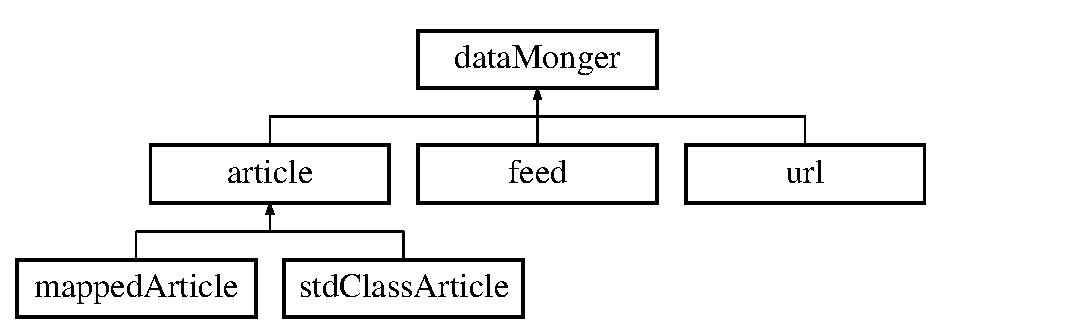
\includegraphics[height=3.000000cm]{classdataMonger}
\end{center}
\end{figure}
\subsection*{Public Member Functions}
\begin{DoxyCompactItemize}
\item 
\hyperlink{classdataMonger_a5ad21a647bfa545e72230192f77d0d63}{dump} ()
\item 
\hyperlink{classdataMonger_ab4392db7fadc4a2a88d17d12e6f4e1b4}{\-\_\-\-\_\-get} (\$name)
\item 
\hyperlink{classdataMonger_a2f44c7904d8576a71622ac923edb5d0f}{json} ()
\end{DoxyCompactItemize}
\subsection*{Protected Attributes}
\begin{DoxyCompactItemize}
\item 
\hypertarget{classdataMonger_aca99065a518f42f3921385dad07b82b2}{{\bfseries \$container}}\label{classdataMonger_aca99065a518f42f3921385dad07b82b2}

\end{DoxyCompactItemize}


\subsection{Detailed Description}
Provides an abstract class for objects to inherit in order to provide a few base functions and a container for contained data. \begin{DoxyAuthor}{Author}
Nate Levesque \href{mailto:public@thenaterhood.com}{\tt public@thenaterhood.\-com} Provides an abstract class to define a standard way of managing data for the classes that are managing things like session data, posts, etc.
\end{DoxyAuthor}
\begin{DoxySince}{Since}
4/13/2013 
\end{DoxySince}


\subsection{Member Function Documentation}
\hypertarget{classdataMonger_ab4392db7fadc4a2a88d17d12e6f4e1b4}{\index{data\-Monger@{data\-Monger}!\-\_\-\-\_\-get@{\-\_\-\-\_\-get}}
\index{\-\_\-\-\_\-get@{\-\_\-\-\_\-get}!dataMonger@{data\-Monger}}
\subsubsection[{\-\_\-\-\_\-get}]{\setlength{\rightskip}{0pt plus 5cm}data\-Monger\-::\-\_\-\-\_\-get (
\begin{DoxyParamCaption}
\item[{}]{\$name}
\end{DoxyParamCaption}
)}}\label{classdataMonger_ab4392db7fadc4a2a88d17d12e6f4e1b4}
Retrieves a field from the container, assuming the container is an associative array.


\begin{DoxyParams}{Parameters}
{\em \$name} & -\/ the item to retrieve \\
\hline
\end{DoxyParams}
\hypertarget{classdataMonger_a5ad21a647bfa545e72230192f77d0d63}{\index{data\-Monger@{data\-Monger}!dump@{dump}}
\index{dump@{dump}!dataMonger@{data\-Monger}}
\subsubsection[{dump}]{\setlength{\rightskip}{0pt plus 5cm}data\-Monger\-::dump (
\begin{DoxyParamCaption}
{}
\end{DoxyParamCaption}
)}}\label{classdataMonger_a5ad21a647bfa545e72230192f77d0d63}
Returns the contents of the container \hypertarget{classdataMonger_a2f44c7904d8576a71622ac923edb5d0f}{\index{data\-Monger@{data\-Monger}!json@{json}}
\index{json@{json}!dataMonger@{data\-Monger}}
\subsubsection[{json}]{\setlength{\rightskip}{0pt plus 5cm}data\-Monger\-::json (
\begin{DoxyParamCaption}
{}
\end{DoxyParamCaption}
)}}\label{classdataMonger_a2f44c7904d8576a71622ac923edb5d0f}
Produces a json encoded representation of the data contained in the class. 

The documentation for this class was generated from the following file\-:\begin{DoxyCompactItemize}
\item 
engine/classes/class\-\_\-data\-Monger.\-php\end{DoxyCompactItemize}

\hypertarget{classengine}{\section{engine Class Reference}
\label{classengine}\index{engine@{engine}}
}
\subsection*{Static Public Member Functions}
\begin{DoxyCompactItemize}
\item 
\hypertarget{classengine_a64c1ff9adad7e9ecc08ff1d832d14f1d}{static {\bfseries handle\-\_\-exception} (\$e)}\label{classengine_a64c1ff9adad7e9ecc08ff1d832d14f1d}

\item 
\hypertarget{classengine_a06db5cb5595cf6e64e3cda77e0c0b4bc}{static {\bfseries get\-\_\-option} (\$option)}\label{classengine_a06db5cb5595cf6e64e3cda77e0c0b4bc}

\end{DoxyCompactItemize}


\subsection{Detailed Description}
Contains internal naterweb functionality for handling some generic internal features such as error handling. 

The documentation for this class was generated from the following file\-:\begin{DoxyCompactItemize}
\item 
engine/classes/class\-\_\-engine.\-php\end{DoxyCompactItemize}

\hypertarget{classErrorStack}{\section{Error\-Stack Class Reference}
\label{classErrorStack}\index{Error\-Stack@{Error\-Stack}}
}
\subsection*{Static Public Member Functions}
\begin{DoxyCompactItemize}
\item 
static \hyperlink{classErrorStack_a20d6f809dbcb58224f5d4fc55b056660}{stack} (\$class=null, \$function=null, \$context=null, \$error\-Code=null)
\item 
static \hyperlink{classErrorStack_a6c3ccaff191e9e24ad88fec0fa13d892}{has\-Error} (\$class=null, \$function=null, \$context=null, \$error\-Code=null)
\item 
\hypertarget{classErrorStack_a0ee37a5d0c2f944f420cc027bf9043d4}{static {\bfseries has\-Error\-With\-Code} (\$code)}\label{classErrorStack_a0ee37a5d0c2f944f420cc027bf9043d4}

\item 
static \hyperlink{classErrorStack_a9fc1e04e762628613015cf62a055d4aa}{errors\-With\-Context} (\$context)
\item 
static \hyperlink{classErrorStack_a670a1b10810e2c230bbe8dc4cb7eca3f}{get\-Message} (\$class, \$function, \$context, \$error\-Code)
\item 
static \hyperlink{classErrorStack_aa1e47d928ad756d6b8fe20bc726ab32e}{get\-Message\-With\-Context} (\$context)
\item 
static \hyperlink{classErrorStack_ae2ee29b47d837e6d59436469593652f3}{add} (\$message, \$class=null, \$function=null, \$variables=array(), \$context=null, \$code=0)
\item 
static \hyperlink{classErrorStack_ad2333eb215c105c406b97bffb814a13c}{set\-Context} (\$context)
\item 
static \hyperlink{classErrorStack_a239a25d7d6616a65cfae42fb0a68d4ab}{clear\-Context} ()
\item 
static \hyperlink{classErrorStack_ad809b79d98533e74b1fa4cc8e3273e9a}{dump} ()
\item 
\hypertarget{classErrorStack_a140907f6dc51528f612170d866bdcff9}{static {\bfseries generate\-Message} (\$message, \$variables=array())}\label{classErrorStack_a140907f6dc51528f612170d866bdcff9}

\end{DoxyCompactItemize}


\subsection{Detailed Description}
Handles the creation and storing of non-\/fatal errors. This class may be useful for logging errors or displaying them to users. \begin{DoxyAuthor}{Author}
Jared King \href{mailto:j@jaredtking.com}{\tt j@jaredtking.\-com} \hyperlink{}{1.\-0  2012 Groupr  M\-I\-T Permission is hereby granted, free of charge, to any person obtaining a copy of this software and associated documentation files (the \char`\"{}\-Software\char`\"{}), to deal in the Software without restriction, including without limitation the rights to use, copy, modify, merge, publish, distribute, sublicense, and/or sell copies of the Software, and to permit persons to whom the Software is furnished to do so, subject to the following conditions\-:  The above copyright notice and this permission notice shall be included in all copies or substantial portions of the Software.  T\-H\-E S\-O\-F\-T\-W\-A\-R\-E I\-S P\-R\-O\-V\-I\-D\-E\-D \char`\"{}\-A\-S I\-S\char`\"{}, W\-I\-T\-H\-O\-U\-T W\-A\-R\-R\-A\-N\-T\-Y O\-F A\-N\-Y K\-I\-N\-D, E\-X\-P\-R\-E\-S\-S O\-R I\-M\-P\-L\-I\-E\-D, I\-N\-C\-L\-U\-D\-I\-N\-G B\-U\-T N\-O\-T L\-I\-M\-I\-T\-E\-D T\-O T\-H\-E W\-A\-R\-R\-A\-N\-T\-I\-E\-S O\-F M\-E\-R\-C\-H\-A\-N\-T\-A\-B\-I\-L\-I\-T\-Y, F\-I\-T\-N\-E\-S\-S F\-O\-R A P\-A\-R\-T\-I\-C\-U\-L\-A\-R P\-U\-R\-P\-O\-S\-E A\-N\-D N\-O\-N\-I\-N\-F\-R\-I\-N\-G\-E\-M\-E\-N\-T. I\-N N\-O E\-V\-E\-N\-T S\-H\-A\-L\-L T\-H\-E A\-U\-T\-H\-O\-R\-S O\-R C\-O\-P\-Y\-R\-I\-G\-H\-T H\-O\-L\-D\-E\-R\-S B\-E L\-I\-A\-B\-L\-E F\-O\-R A\-N\-Y C\-L\-A\-I\-M, D\-A\-M\-A\-G\-E\-S O\-R O\-T\-H\-E\-R L\-I\-A\-B\-I\-L\-I\-T\-Y, W\-H\-E\-T\-H\-E\-R I\-N A\-N A\-C\-T\-I\-O\-N O\-F C\-O\-N\-T\-R\-A\-C\-T, T\-O\-R\-T O\-R O\-T\-H\-E\-R\-W\-I\-S\-E, A\-R\-I\-S\-I\-N\-G F\-R\-O\-M, O\-U\-T O\-F O\-R I\-N C\-O\-N\-N\-E\-C\-T\-I\-O\-N W\-I\-T\-H T\-H\-E S\-O\-F\-T\-W\-A\-R\-E O\-R T\-H\-E U\-S\-E O\-R O\-T\-H\-E\-R D\-E\-A\-L\-I\-N\-G\-S I\-N T\-H\-E S\-O\-F\-T\-W\-A\-R\-E. }
\end{DoxyAuthor}


\subsection{Member Function Documentation}
\hypertarget{classErrorStack_ae2ee29b47d837e6d59436469593652f3}{\index{Error\-Stack@{Error\-Stack}!add@{add}}
\index{add@{add}!ErrorStack@{Error\-Stack}}
\subsubsection[{add}]{\setlength{\rightskip}{0pt plus 5cm}static Error\-Stack\-::add (
\begin{DoxyParamCaption}
\item[{}]{\$message, }
\item[{}]{\$class = {\ttfamily null}, }
\item[{}]{\$function = {\ttfamily null}, }
\item[{}]{\$variables = {\ttfamily array()}, }
\item[{}]{\$context = {\ttfamily null}, }
\item[{}]{\$code = {\ttfamily 0}}
\end{DoxyParamCaption}
)\hspace{0.3cm}{\ttfamily [static]}}}\label{classErrorStack_ae2ee29b47d837e6d59436469593652f3}
Adds an error message to the stack


\begin{DoxyParams}[1]{Parameters}
string & {\em \$message} & message \\
\hline
string & {\em \$class} & class \\
\hline
string & {\em \$function} & function \\
\hline
string & {\em \$context} & context \\
\hline
string & {\em \$code} & error code\\
\hline
\end{DoxyParams}
\begin{DoxyReturn}{Returns}
boolean true if successful 
\end{DoxyReturn}
\hypertarget{classErrorStack_a239a25d7d6616a65cfae42fb0a68d4ab}{\index{Error\-Stack@{Error\-Stack}!clear\-Context@{clear\-Context}}
\index{clear\-Context@{clear\-Context}!ErrorStack@{Error\-Stack}}
\subsubsection[{clear\-Context}]{\setlength{\rightskip}{0pt plus 5cm}static Error\-Stack\-::clear\-Context (
\begin{DoxyParamCaption}
{}
\end{DoxyParamCaption}
)\hspace{0.3cm}{\ttfamily [static]}}}\label{classErrorStack_a239a25d7d6616a65cfae42fb0a68d4ab}
Clears the error context

\begin{DoxyReturn}{Returns}
null 
\end{DoxyReturn}
\hypertarget{classErrorStack_ad809b79d98533e74b1fa4cc8e3273e9a}{\index{Error\-Stack@{Error\-Stack}!dump@{dump}}
\index{dump@{dump}!ErrorStack@{Error\-Stack}}
\subsubsection[{dump}]{\setlength{\rightskip}{0pt plus 5cm}static Error\-Stack\-::dump (
\begin{DoxyParamCaption}
{}
\end{DoxyParamCaption}
)\hspace{0.3cm}{\ttfamily [static]}}}\label{classErrorStack_ad809b79d98533e74b1fa4cc8e3273e9a}
Prints out the error stack (for debugging) \hypertarget{classErrorStack_a9fc1e04e762628613015cf62a055d4aa}{\index{Error\-Stack@{Error\-Stack}!errors\-With\-Context@{errors\-With\-Context}}
\index{errors\-With\-Context@{errors\-With\-Context}!ErrorStack@{Error\-Stack}}
\subsubsection[{errors\-With\-Context}]{\setlength{\rightskip}{0pt plus 5cm}static Error\-Stack\-::errors\-With\-Context (
\begin{DoxyParamCaption}
\item[{}]{\$context}
\end{DoxyParamCaption}
)\hspace{0.3cm}{\ttfamily [static]}}}\label{classErrorStack_a9fc1e04e762628613015cf62a055d4aa}
Finds errors based on the given parameters


\begin{DoxyParams}[1]{Parameters}
string & {\em \$context} & error context\\
\hline
\end{DoxyParams}
\begin{DoxyReturn}{Returns}
array 
\end{DoxyReturn}
\hypertarget{classErrorStack_a670a1b10810e2c230bbe8dc4cb7eca3f}{\index{Error\-Stack@{Error\-Stack}!get\-Message@{get\-Message}}
\index{get\-Message@{get\-Message}!ErrorStack@{Error\-Stack}}
\subsubsection[{get\-Message}]{\setlength{\rightskip}{0pt plus 5cm}static Error\-Stack\-::get\-Message (
\begin{DoxyParamCaption}
\item[{}]{\$class, }
\item[{}]{\$function, }
\item[{}]{\$context, }
\item[{}]{\$error\-Code}
\end{DoxyParamCaption}
)\hspace{0.3cm}{\ttfamily [static]}}}\label{classErrorStack_a670a1b10810e2c230bbe8dc4cb7eca3f}
Gets a single (first) message based on the given parameters.

If multiple errors are matched then only the first one will be returned. If more than one error is possible it is best to user the \hyperlink{classErrorStack_a20d6f809dbcb58224f5d4fc55b056660}{stack()} method


\begin{DoxyParams}[1]{Parameters}
string & {\em \$class} & class \\
\hline
string & {\em \$function} & function \\
\hline
string & {\em \$context} & context \\
\hline
string | int & {\em \$error\-Code} & error code\\
\hline
\end{DoxyParams}
\begin{DoxyReturn}{Returns}
string message 
\end{DoxyReturn}
\hypertarget{classErrorStack_aa1e47d928ad756d6b8fe20bc726ab32e}{\index{Error\-Stack@{Error\-Stack}!get\-Message\-With\-Context@{get\-Message\-With\-Context}}
\index{get\-Message\-With\-Context@{get\-Message\-With\-Context}!ErrorStack@{Error\-Stack}}
\subsubsection[{get\-Message\-With\-Context}]{\setlength{\rightskip}{0pt plus 5cm}static Error\-Stack\-::get\-Message\-With\-Context (
\begin{DoxyParamCaption}
\item[{}]{\$context}
\end{DoxyParamCaption}
)\hspace{0.3cm}{\ttfamily [static]}}}\label{classErrorStack_aa1e47d928ad756d6b8fe20bc726ab32e}
Gets the first message from the error stack for a given context


\begin{DoxyParams}[1]{Parameters}
string & {\em \$context} & context\\
\hline
\end{DoxyParams}
\begin{DoxyReturn}{Returns}
string message 
\end{DoxyReturn}
\hypertarget{classErrorStack_a6c3ccaff191e9e24ad88fec0fa13d892}{\index{Error\-Stack@{Error\-Stack}!has\-Error@{has\-Error}}
\index{has\-Error@{has\-Error}!ErrorStack@{Error\-Stack}}
\subsubsection[{has\-Error}]{\setlength{\rightskip}{0pt plus 5cm}static Error\-Stack\-::has\-Error (
\begin{DoxyParamCaption}
\item[{}]{\$class = {\ttfamily null}, }
\item[{}]{\$function = {\ttfamily null}, }
\item[{}]{\$context = {\ttfamily null}, }
\item[{}]{\$error\-Code = {\ttfamily null}}
\end{DoxyParamCaption}
)\hspace{0.3cm}{\ttfamily [static]}}}\label{classErrorStack_a6c3ccaff191e9e24ad88fec0fa13d892}
Checks if an error exists based on the given parameters.


\begin{DoxyParams}[1]{Parameters}
string & {\em \$class} & class \\
\hline
string & {\em \$function} & function \\
\hline
string & {\em \$context} & context \\
\hline
string | int & {\em \$error\-Code} & error code\\
\hline
\end{DoxyParams}
\begin{DoxyReturn}{Returns}
boolean true if at least one error exists 
\end{DoxyReturn}
\hypertarget{classErrorStack_ad2333eb215c105c406b97bffb814a13c}{\index{Error\-Stack@{Error\-Stack}!set\-Context@{set\-Context}}
\index{set\-Context@{set\-Context}!ErrorStack@{Error\-Stack}}
\subsubsection[{set\-Context}]{\setlength{\rightskip}{0pt plus 5cm}static Error\-Stack\-::set\-Context (
\begin{DoxyParamCaption}
\item[{}]{\$context}
\end{DoxyParamCaption}
)\hspace{0.3cm}{\ttfamily [static]}}}\label{classErrorStack_ad2333eb215c105c406b97bffb814a13c}
Sets the context for all errors created.

Unless explicitly overridden all errors will be created with the current context. Don't forget to clear the context when finished with it.


\begin{DoxyParams}{Parameters}
{\em string} & context\\
\hline
\end{DoxyParams}
\begin{DoxyReturn}{Returns}
null 
\end{DoxyReturn}
\hypertarget{classErrorStack_a20d6f809dbcb58224f5d4fc55b056660}{\index{Error\-Stack@{Error\-Stack}!stack@{stack}}
\index{stack@{stack}!ErrorStack@{Error\-Stack}}
\subsubsection[{stack}]{\setlength{\rightskip}{0pt plus 5cm}static Error\-Stack\-::stack (
\begin{DoxyParamCaption}
\item[{}]{\$class = {\ttfamily null}, }
\item[{}]{\$function = {\ttfamily null}, }
\item[{}]{\$context = {\ttfamily null}, }
\item[{}]{\$error\-Code = {\ttfamily null}}
\end{DoxyParamCaption}
)\hspace{0.3cm}{\ttfamily [static]}}}\label{classErrorStack_a20d6f809dbcb58224f5d4fc55b056660}
Gets error(s) in the stack based on the desired parameters

This method is useful for pulling errors off the stack that occured within a class, function, context, by error code or any combination of these parameters.


\begin{DoxyParams}[1]{Parameters}
string & {\em \$class} & class (optional) \\
\hline
string & {\em \$function} & function (optional) \\
\hline
string & {\em \$context} & context (optional) \\
\hline
string | int & {\em \$error\-Code} & error code (optional)\\
\hline
\end{DoxyParams}
\begin{DoxyReturn}{Returns}
array errors 
\end{DoxyReturn}


The documentation for this class was generated from the following file\-:\begin{DoxyCompactItemize}
\item 
engine/lib/extern/php-\/database/Error\-Stack.\-php\end{DoxyCompactItemize}

\hypertarget{interfaceExtension}{\section{Extension Interface Reference}
\label{interfaceExtension}\index{Extension@{Extension}}
}
\subsection*{Public Member Functions}
\begin{DoxyCompactItemize}
\item 
\hypertarget{interfaceExtension_aad71d40510cdd0419880b8d0ca69b60b}{{\bfseries \-\_\-\-\_\-construct} (\$session)}\label{interfaceExtension_aad71d40510cdd0419880b8d0ca69b60b}

\item 
\hypertarget{interfaceExtension_a33fb91d202931e147dcd7ca687335c85}{{\bfseries get\-Preface\-Code} ()}\label{interfaceExtension_a33fb91d202931e147dcd7ca687335c85}

\item 
\hypertarget{interfaceExtension_aeef8c20babee8dc0177b3bf4e13cf2df}{{\bfseries get\-Post\-Code} ()}\label{interfaceExtension_aeef8c20babee8dc0177b3bf4e13cf2df}

\end{DoxyCompactItemize}


The documentation for this interface was generated from the following file\-:\begin{DoxyCompactItemize}
\item 
engine/classes/interface\-\_\-extension.\-php\end{DoxyCompactItemize}

\hypertarget{classfeed}{\section{feed Class Reference}
\label{classfeed}\index{feed@{feed}}
}
Inheritance diagram for feed\-:\begin{figure}[H]
\begin{center}
\leavevmode
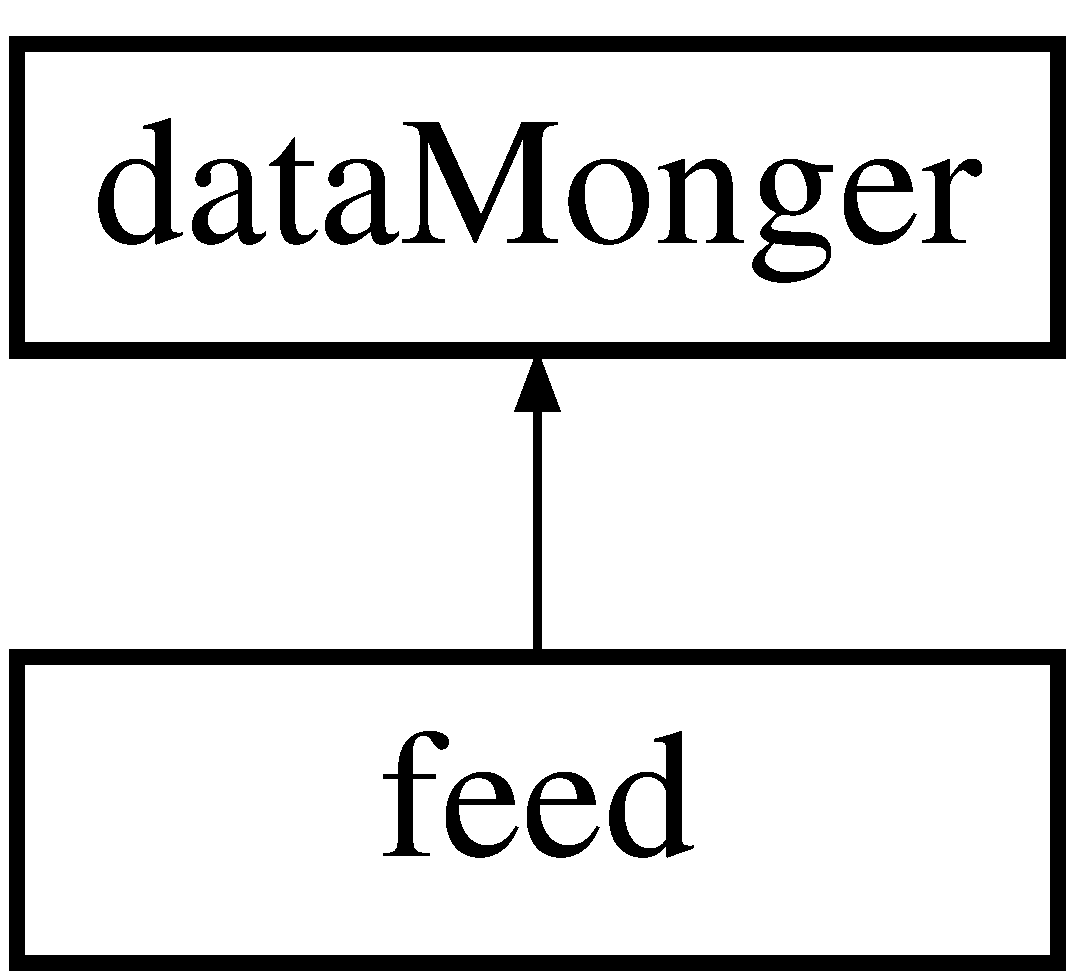
\includegraphics[height=2.000000cm]{classfeed}
\end{center}
\end{figure}
\subsection*{Public Member Functions}
\begin{DoxyCompactItemize}
\item 
\hyperlink{classfeed_af02c4453c03c206d203baaf0a4361e0c}{\-\_\-\-\_\-construct} (\$title, \$link, \$description, \$feedstamp)
\item 
\hyperlink{classfeed_a470f18a51bf971b23d3ff2881bbb58a0}{new\-\_\-item} (\$articleect)
\item 
\hyperlink{classfeed_a0c5547688b01b08cb78a58ff62f70444}{output} (\$type)
\end{DoxyCompactItemize}
\subsection*{Additional Inherited Members}


\subsection{Detailed Description}
Provides a resource for building an rss or atom feed. Include the inherited \hyperlink{classdataMonger}{data\-Monger} class Defines a data object to contain an atom feed as items are added and the feed is updated then returned 

\subsection{Constructor \& Destructor Documentation}
\hypertarget{classfeed_af02c4453c03c206d203baaf0a4361e0c}{\index{feed@{feed}!\-\_\-\-\_\-construct@{\-\_\-\-\_\-construct}}
\index{\-\_\-\-\_\-construct@{\-\_\-\-\_\-construct}!feed@{feed}}
\subsubsection[{\-\_\-\-\_\-construct}]{\setlength{\rightskip}{0pt plus 5cm}feed\-::\-\_\-\-\_\-construct (
\begin{DoxyParamCaption}
\item[{}]{\$title, }
\item[{}]{\$link, }
\item[{}]{\$description, }
\item[{}]{\$feedstamp}
\end{DoxyParamCaption}
)}}\label{classfeed_af02c4453c03c206d203baaf0a4361e0c}
Creates an empty atom feed object with metadata


\begin{DoxyParams}{Parameters}
{\em \$title} & (str)\-: a title for the atom feed \\
\hline
{\em \$link} & (str)\-: the base url for the feed \\
\hline
{\em \$description} & (str)\-: a description or summary of the feed \\
\hline
{\em \$feedstamp} & (str)\-: a datestamp for the feed, in standard atom format \\
\hline
\end{DoxyParams}


\subsection{Member Function Documentation}
\hypertarget{classfeed_a470f18a51bf971b23d3ff2881bbb58a0}{\index{feed@{feed}!new\-\_\-item@{new\-\_\-item}}
\index{new\-\_\-item@{new\-\_\-item}!feed@{feed}}
\subsubsection[{new\-\_\-item}]{\setlength{\rightskip}{0pt plus 5cm}feed\-::new\-\_\-item (
\begin{DoxyParamCaption}
\item[{}]{\$articleect}
\end{DoxyParamCaption}
)}}\label{classfeed_a470f18a51bf971b23d3ff2881bbb58a0}
Adds an item to the feed as an object in the object's items array


\begin{DoxyParams}{Parameters}
{\em \$articleect} & -\/ a fully initialized instance of the article class. \\
\hline
\end{DoxyParams}
\hypertarget{classfeed_a0c5547688b01b08cb78a58ff62f70444}{\index{feed@{feed}!output@{output}}
\index{output@{output}!feed@{feed}}
\subsubsection[{output}]{\setlength{\rightskip}{0pt plus 5cm}feed\-::output (
\begin{DoxyParamCaption}
\item[{}]{\$type}
\end{DoxyParamCaption}
)}}\label{classfeed_a0c5547688b01b08cb78a58ff62f70444}
Returns a valid feed with the requested format.


\begin{DoxyParams}{Parameters}
{\em \$type} & -\/ the type of feed to return (atom/rss). Defaults to atom (superior) if the type given not recognized. \\
\hline
\end{DoxyParams}


The documentation for this class was generated from the following file\-:\begin{DoxyCompactItemize}
\item 
engine/classes/class\-\_\-feed.\-php\end{DoxyCompactItemize}

\hypertarget{classfeeds}{\section{feeds Class Reference}
\label{classfeeds}\index{feeds@{feeds}}
}
Inheritance diagram for feeds\-:\begin{figure}[H]
\begin{center}
\leavevmode
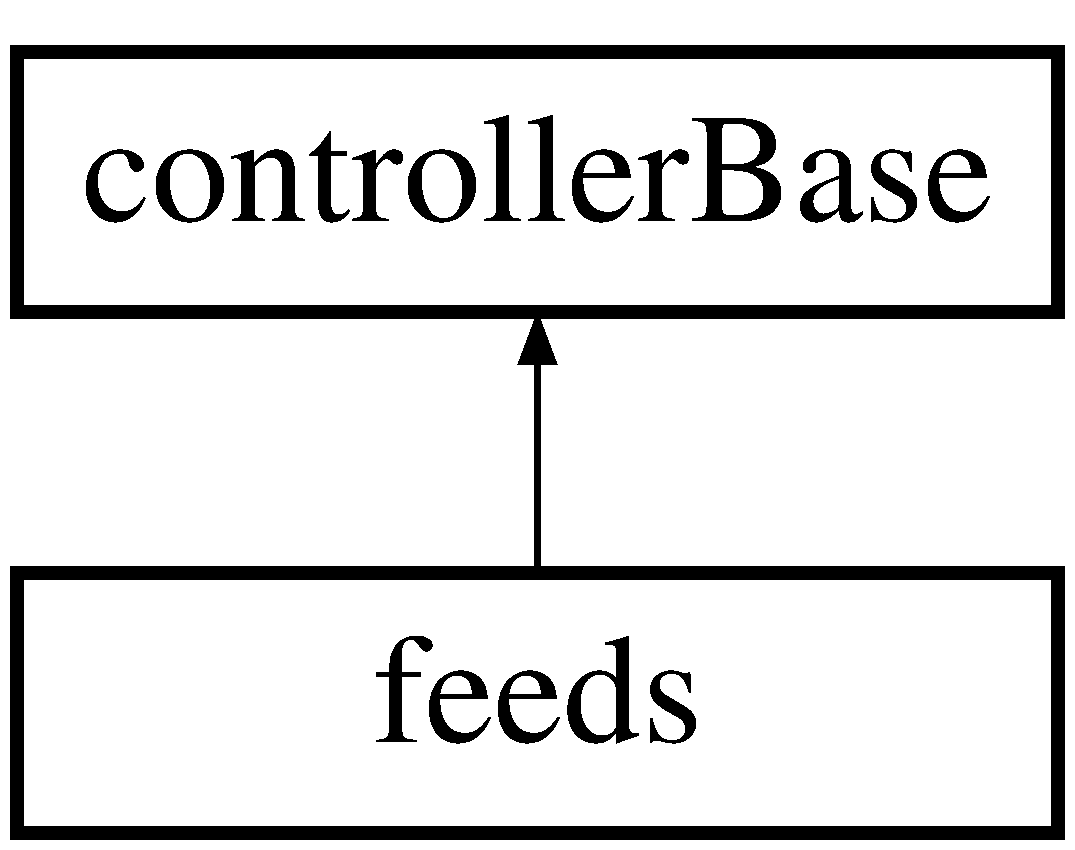
\includegraphics[height=2.000000cm]{classfeeds}
\end{center}
\end{figure}
\subsection*{Public Member Functions}
\begin{DoxyCompactItemize}
\item 
\hypertarget{classfeeds_a78a1e45b9170c42ac091d9395770a391}{{\bfseries \-\_\-\-\_\-call} (\$method, \$args)}\label{classfeeds_a78a1e45b9170c42ac091d9395770a391}

\end{DoxyCompactItemize}
\subsection*{Additional Inherited Members}


The documentation for this class was generated from the following file\-:\begin{DoxyCompactItemize}
\item 
engine/lib/builtins/feeds/main.\-php\end{DoxyCompactItemize}

\hypertarget{classFile}{\section{File Class Reference}
\label{classFile}\index{File@{File}}
}
\subsection*{Public Member Functions}
\begin{DoxyCompactItemize}
\item 
\hypertarget{classFile_a7c30c00c75307f63ba64a6dfc51bdf40}{{\bfseries \-\_\-\-\_\-construct} (\$name, \$type=null)}\label{classFile_a7c30c00c75307f63ba64a6dfc51bdf40}

\item 
\hypertarget{classFile_a335b354b4bdc037234819672ef748a6a}{{\bfseries get\-\_\-contents} ()}\label{classFile_a335b354b4bdc037234819672ef748a6a}

\item 
\hypertarget{classFile_a690e235b49fc3edd286c06b8c3c45dc6}{{\bfseries read\-\_\-as\-\_\-json} ()}\label{classFile_a690e235b49fc3edd286c06b8c3c45dc6}

\item 
\hypertarget{classFile_aa5079110853e078baf343d4c14d008ef}{{\bfseries search\-For\-File} ()}\label{classFile_aa5079110853e078baf343d4c14d008ef}

\item 
\hypertarget{classFile_a54a61b7b4554eadc8152308e0ba818fa}{{\bfseries get\-Lock} ()}\label{classFile_a54a61b7b4554eadc8152308e0ba818fa}

\item 
\hypertarget{classFile_ab407397f208a0ea253b877f0ea35a224}{{\bfseries clear} ()}\label{classFile_ab407397f208a0ea253b877f0ea35a224}

\item 
\hypertarget{classFile_a0abbca3d8b81e29f01db75ec19d0ef84}{{\bfseries delete} ()}\label{classFile_a0abbca3d8b81e29f01db75ec19d0ef84}

\item 
\hypertarget{classFile_acf33002bc9fe7e7a2d965b7c2da6a153}{{\bfseries append} (\$string)}\label{classFile_acf33002bc9fe7e7a2d965b7c2da6a153}

\item 
\hypertarget{classFile_af75690cb66613f6086f7fa9a16b0a710}{{\bfseries overwrite} (\$string)}\label{classFile_af75690cb66613f6086f7fa9a16b0a710}

\item 
\hypertarget{classFile_ac2605a992d142fbb5b1dfcc214871e35}{{\bfseries save} ()}\label{classFile_ac2605a992d142fbb5b1dfcc214871e35}

\item 
\hypertarget{classFile_a5a5183f2549633a2804b24b8eee36e23}{{\bfseries \-\_\-\-\_\-destroy} ()}\label{classFile_a5a5183f2549633a2804b24b8eee36e23}

\end{DoxyCompactItemize}


The documentation for this class was generated from the following file\-:\begin{DoxyCompactItemize}
\item 
engine/classes/class\-\_\-file.\-php\end{DoxyCompactItemize}

\hypertarget{classlock}{\section{lock Class Reference}
\label{classlock}\index{lock@{lock}}
}
\subsection*{Public Member Functions}
\begin{DoxyCompactItemize}
\item 
\hyperlink{classlock_a2b1318e68e5f10a8e87ea653023f4966}{\-\_\-\-\_\-construct} (\$file)
\item 
\hyperlink{classlock_a8a4d0c241ded71bb02dbdf9b26e759dd}{is\-Locked} ()
\item 
\hyperlink{classlock_a50f07760e0ecc88f17310b820d38e7e3}{lock} ()
\item 
\hyperlink{classlock_af3a6ea9d4064b261a59a0760dc42980c}{unlock} ()
\end{DoxyCompactItemize}


\subsection{Detailed Description}
Contains a class that deals with managing file locks Include the config class so we can retrieve the dynamic directory Defines a class to manage locks for files \begin{DoxySince}{Since}
06/05/2013 
\end{DoxySince}
\begin{DoxyAuthor}{Author}
Nate Levesque \href{mailto:public@thenaterhood.com}{\tt public@thenaterhood.\-com} 
\end{DoxyAuthor}


\subsection{Constructor \& Destructor Documentation}
\hypertarget{classlock_a2b1318e68e5f10a8e87ea653023f4966}{\index{lock@{lock}!\-\_\-\-\_\-construct@{\-\_\-\-\_\-construct}}
\index{\-\_\-\-\_\-construct@{\-\_\-\-\_\-construct}!lock@{lock}}
\subsubsection[{\-\_\-\-\_\-construct}]{\setlength{\rightskip}{0pt plus 5cm}lock\-::\-\_\-\-\_\-construct (
\begin{DoxyParamCaption}
\item[{}]{\$file}
\end{DoxyParamCaption}
)}}\label{classlock_a2b1318e68e5f10a8e87ea653023f4966}
Constructs and instance of the lock class 
\begin{DoxyParams}{Parameters}
{\em \$file} & -\/ the file (full path) to create a lock for \\
\hline
\end{DoxyParams}


\subsection{Member Function Documentation}
\hypertarget{classlock_a8a4d0c241ded71bb02dbdf9b26e759dd}{\index{lock@{lock}!is\-Locked@{is\-Locked}}
\index{is\-Locked@{is\-Locked}!lock@{lock}}
\subsubsection[{is\-Locked}]{\setlength{\rightskip}{0pt plus 5cm}lock\-::is\-Locked (
\begin{DoxyParamCaption}
{}
\end{DoxyParamCaption}
)}}\label{classlock_a8a4d0c241ded71bb02dbdf9b26e759dd}
Returns whether or not the file has been locked \begin{DoxyReturn}{Returns}
-\/ boolean True if a lock exists 
\end{DoxyReturn}
\hypertarget{classlock_a50f07760e0ecc88f17310b820d38e7e3}{\index{lock@{lock}!lock@{lock}}
\index{lock@{lock}!lock@{lock}}
\subsubsection[{lock}]{\setlength{\rightskip}{0pt plus 5cm}lock\-::lock (
\begin{DoxyParamCaption}
{}
\end{DoxyParamCaption}
)}}\label{classlock_a50f07760e0ecc88f17310b820d38e7e3}
Creates a lock for the file in the dynamic directory. Note that for this to be effective, everything must actually observe locks. \hypertarget{classlock_af3a6ea9d4064b261a59a0760dc42980c}{\index{lock@{lock}!unlock@{unlock}}
\index{unlock@{unlock}!lock@{lock}}
\subsubsection[{unlock}]{\setlength{\rightskip}{0pt plus 5cm}lock\-::unlock (
\begin{DoxyParamCaption}
{}
\end{DoxyParamCaption}
)}}\label{classlock_af3a6ea9d4064b261a59a0760dc42980c}
Removes a lock on a file 

The documentation for this class was generated from the following file\-:\begin{DoxyCompactItemize}
\item 
engine/classes/class\-\_\-lock.\-php\end{DoxyCompactItemize}

\hypertarget{classmappedArticle}{\section{mapped\-Article Class Reference}
\label{classmappedArticle}\index{mapped\-Article@{mapped\-Article}}
}
Inheritance diagram for mapped\-Article\-:\begin{figure}[H]
\begin{center}
\leavevmode
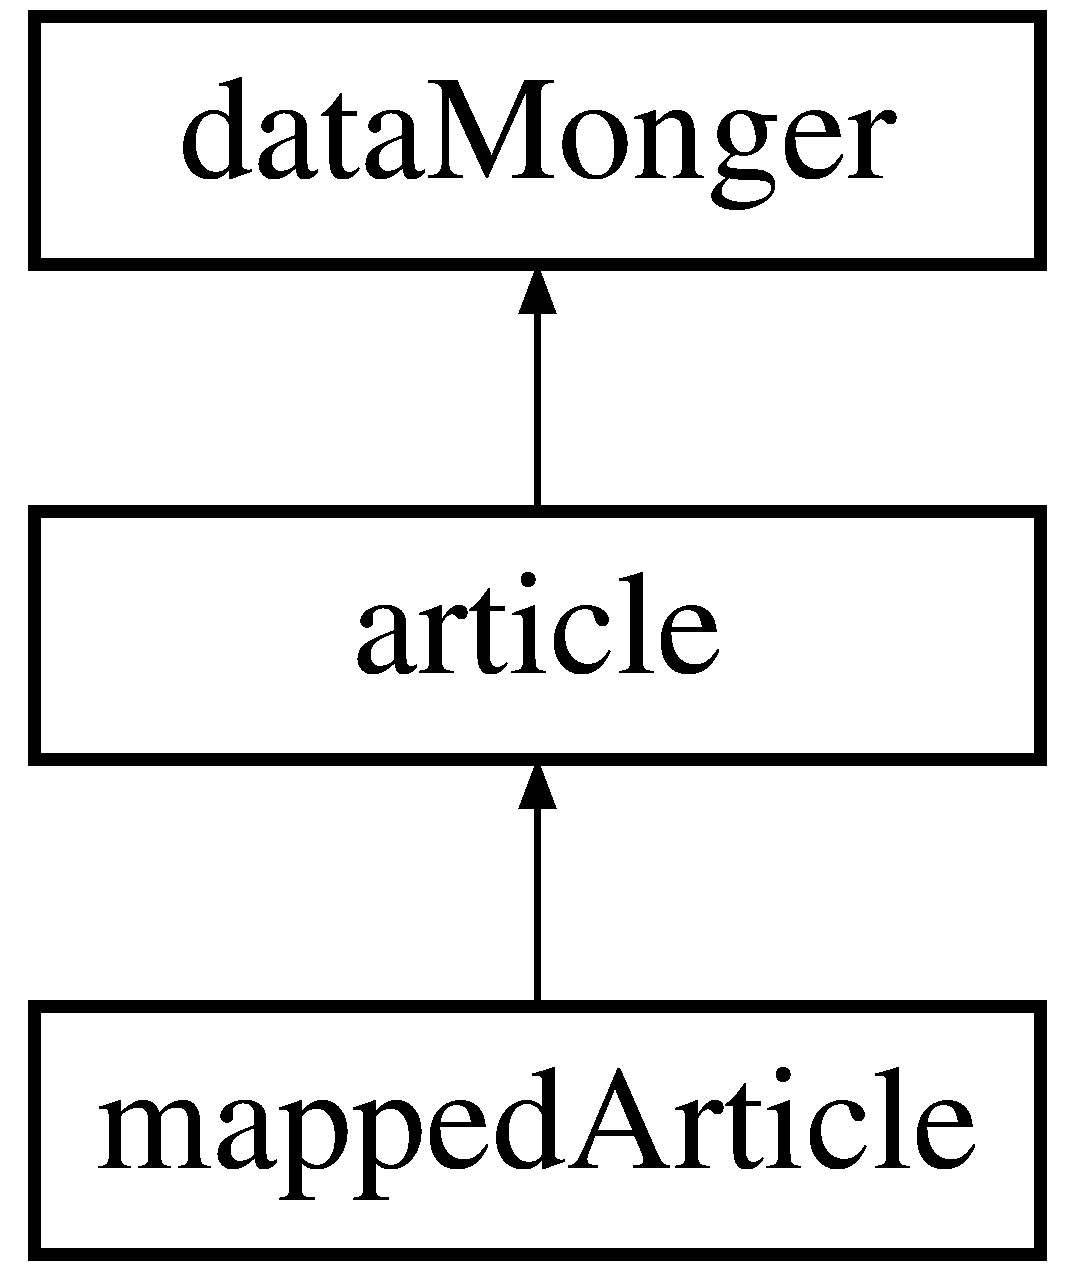
\includegraphics[height=3.000000cm]{classmappedArticle}
\end{center}
\end{figure}
\subsection*{Public Member Functions}
\begin{DoxyCompactItemize}
\item 
\hypertarget{classmappedArticle_a1eba5bad9e5365838d33070dda0cddd3}{{\bfseries \-\_\-\-\_\-construct} (\$map, \$post\-Format=False)}\label{classmappedArticle_a1eba5bad9e5365838d33070dda0cddd3}

\end{DoxyCompactItemize}
\subsection*{Additional Inherited Members}


The documentation for this class was generated from the following file\-:\begin{DoxyCompactItemize}
\item 
engine/classes/class\-\_\-mapped\-Article.\-php\end{DoxyCompactItemize}

\hypertarget{classModel}{\section{Model Class Reference}
\label{classModel}\index{Model@{Model}}
}
\subsection*{Static Public Member Functions}
\begin{DoxyCompactItemize}
\item 
\hypertarget{classModel_ab9216a19669cfe36185f2708614b3f3b}{static {\bfseries Integer\-Field} (\$attrs=array())}\label{classModel_ab9216a19669cfe36185f2708614b3f3b}

\item 
\hypertarget{classModel_a816f494f0a76785786665c500ef957c3}{static {\bfseries Validate\-Integer\-Field} (\$field\-Inst)}\label{classModel_a816f494f0a76785786665c500ef957c3}

\item 
\hypertarget{classModel_a60ca6a2e46ac811b5e48de736fe7a9e6}{static {\bfseries Text\-Field} (\$attrs=array())}\label{classModel_a60ca6a2e46ac811b5e48de736fe7a9e6}

\item 
\hypertarget{classModel_a736897403db67297bc3eb89076858224}{static {\bfseries Validate\-Text\-Field} (\$field\-Inst)}\label{classModel_a736897403db67297bc3eb89076858224}

\item 
\hypertarget{classModel_ad309e7380233caa60a452a835d6efd79}{static {\bfseries Char\-Field} (\$attrs=array())}\label{classModel_ad309e7380233caa60a452a835d6efd79}

\item 
\hypertarget{classModel_ae825ee44bd2b96749b4cdc9f7749c036}{static {\bfseries Validate\-Char\-Field} (\$fieldinst)}\label{classModel_ae825ee44bd2b96749b4cdc9f7749c036}

\item 
\hypertarget{classModel_aef711c224262aeae7d118247bc63ac94}{static {\bfseries Foreign\-Key} (\$attrs=array())}\label{classModel_aef711c224262aeae7d118247bc63ac94}

\item 
\hypertarget{classModel_a0059b7ec64cc31e4bb8f8bc9ff6bd5b1}{static {\bfseries Validate\-Foreign\-Key} (\$fieldinst)}\label{classModel_a0059b7ec64cc31e4bb8f8bc9ff6bd5b1}

\item 
\hypertarget{classModel_a3f4ddd94949057b39165ef27a1a8e1a6}{static {\bfseries Many\-To\-Many} (\$attrs=array())}\label{classModel_a3f4ddd94949057b39165ef27a1a8e1a6}

\item 
\hypertarget{classModel_af47f078690e96ef2602b7c3a6c68255e}{static {\bfseries Boolean\-Field} (\$attrs=array())}\label{classModel_af47f078690e96ef2602b7c3a6c68255e}

\item 
\hypertarget{classModel_aa6389e275a5d6206eb6bea93b72c1b2b}{static {\bfseries Validate\-Boolean\-Field} (\$fieldinst)}\label{classModel_aa6389e275a5d6206eb6bea93b72c1b2b}

\end{DoxyCompactItemize}


The documentation for this class was generated from the following file\-:\begin{DoxyCompactItemize}
\item 
engine/classes/class\-\_\-model.\-php\end{DoxyCompactItemize}

\hypertarget{classModelBase}{\section{Model\-Base Class Reference}
\label{classModelBase}\index{Model\-Base@{Model\-Base}}
}
\subsection*{Public Member Functions}
\begin{DoxyCompactItemize}
\item 
\hyperlink{classModelBase_afe2a0077074c8fd54372fae3461919b9}{save} ()
\item 
\hyperlink{classModelBase_a5183135ede8664baa606dbdf9fc2eca0}{delete} ()
\item 
\hyperlink{classModelBase_a1b3373e9cf5d2920528a0c46ddc7c42f}{\-\_\-\-\_\-get} (\$field)
\item 
\hyperlink{classModelBase_ae19b572d12d6a9d9e64556ec6b7a9c25}{get\-Related} (\$name)
\item 
\hyperlink{classModelBase_ad820af9bc876f247be8e15b44c8b4dc4}{set\-Related} (\$name, \$value)
\item 
\hyperlink{classModelBase_ac93115f1d4999b56db948a4097c978d0}{add\-Related} (\$name, \$value)
\item 
\hyperlink{classModelBase_a48e09bdaa1f60c48ccb73c13eca2e005}{remove\-Related} (\$name, \$value)
\item 
\hyperlink{classModelBase_a012bbaca3aa24a5c7f4ccd5f1c75999c}{\-\_\-\-\_\-set} (\$field, \$value)
\item 
\hyperlink{classModelBase_a8e1e93de9f1c2541ac66777e5513f34a}{get\-Fields} ()
\item 
\hyperlink{classModelBase_ae513caa9e2aa259e42e50003eb4de60a}{as\-\_\-array} ()
\end{DoxyCompactItemize}
\subsection*{Static Public Member Functions}
\begin{DoxyCompactItemize}
\item 
static \hyperlink{classModelBase_adffcc978a896a9f1c3dfc4cfbaf5202b}{from\-Array} (\$array)
\item 
static \hyperlink{classModelBase_a081976e021449729e21eea556201121e}{from\-Std\-Class} (\$class)
\end{DoxyCompactItemize}
\subsection*{Public Attributes}
\begin{DoxyCompactItemize}
\item 
\hypertarget{classModelBase_ac42d971c4d431e98db55742730696bc2}{{\bfseries \$fields} = array()}\label{classModelBase_ac42d971c4d431e98db55742730696bc2}

\end{DoxyCompactItemize}
\subsection*{Protected Member Functions}
\begin{DoxyCompactItemize}
\item 
\hyperlink{classModelBase_a8ada673c0c2e218c9f1c4f6b35c2c9e2}{addfield} (\$name, \$object)
\end{DoxyCompactItemize}
\subsection*{Protected Attributes}
\begin{DoxyCompactItemize}
\item 
\hypertarget{classModelBase_a390c124a3bed604cdf7aa80796d4229e}{{\bfseries \$container}}\label{classModelBase_a390c124a3bed604cdf7aa80796d4229e}

\end{DoxyCompactItemize}


\subsection{Detailed Description}
Include the main model field types class. 

\subsection{Member Function Documentation}
\hypertarget{classModelBase_a1b3373e9cf5d2920528a0c46ddc7c42f}{\index{Model\-Base@{Model\-Base}!\-\_\-\-\_\-get@{\-\_\-\-\_\-get}}
\index{\-\_\-\-\_\-get@{\-\_\-\-\_\-get}!ModelBase@{Model\-Base}}
\subsubsection[{\-\_\-\-\_\-get}]{\setlength{\rightskip}{0pt plus 5cm}Model\-Base\-::\-\_\-\-\_\-get (
\begin{DoxyParamCaption}
\item[{}]{\$field}
\end{DoxyParamCaption}
)}}\label{classModelBase_a1b3373e9cf5d2920528a0c46ddc7c42f}
Retrieves data from the model and returns it. This is necessary as data is contained in the field instances in the model and isn't directly available. Returns the data or the id of the object.


\begin{DoxyParams}{Parameters}
{\em \$field} & -\/ the field of the model to return data for\\
\hline
\end{DoxyParams}
\begin{DoxyReturn}{Returns}
-\/ the data contained in the field
\end{DoxyReturn}

\begin{DoxyExceptions}{Exceptions}
{\em Exception} & -\/ throws an exception if the model field does not exist. \\
\hline
\end{DoxyExceptions}
\hypertarget{classModelBase_a012bbaca3aa24a5c7f4ccd5f1c75999c}{\index{Model\-Base@{Model\-Base}!\-\_\-\-\_\-set@{\-\_\-\-\_\-set}}
\index{\-\_\-\-\_\-set@{\-\_\-\-\_\-set}!ModelBase@{Model\-Base}}
\subsubsection[{\-\_\-\-\_\-set}]{\setlength{\rightskip}{0pt plus 5cm}Model\-Base\-::\-\_\-\-\_\-set (
\begin{DoxyParamCaption}
\item[{}]{\$field, }
\item[{}]{\$value}
\end{DoxyParamCaption}
)}}\label{classModelBase_a012bbaca3aa24a5c7f4ccd5f1c75999c}
Sets the data for a field in the model. This is required as data is stored internally in instances of fields rather than directly in a container or as properties.


\begin{DoxyParams}{Parameters}
{\em \$field} & -\/ the field name to set data for \\
\hline
{\em \$value} & -\/ the data to set\\
\hline
\end{DoxyParams}

\begin{DoxyExceptions}{Exceptions}
{\em Exception} & -\/ throws an exception if the model field does not exist in the model. \\
\hline
\end{DoxyExceptions}
\hypertarget{classModelBase_a8ada673c0c2e218c9f1c4f6b35c2c9e2}{\index{Model\-Base@{Model\-Base}!addfield@{addfield}}
\index{addfield@{addfield}!ModelBase@{Model\-Base}}
\subsubsection[{addfield}]{\setlength{\rightskip}{0pt plus 5cm}Model\-Base\-::addfield (
\begin{DoxyParamCaption}
\item[{}]{\$name, }
\item[{}]{\$object}
\end{DoxyParamCaption}
)\hspace{0.3cm}{\ttfamily [protected]}}}\label{classModelBase_a8ada673c0c2e218c9f1c4f6b35c2c9e2}
Adds a field to the model. This is intended to be called in the constructor of the classes that inherit this class in order to register the fields and relational functionality with the class and the data access layer. Adding fields dynamically is not supported, so adding columns to the database after the model has been registered with the data access layer the first time needs to be done manually.


\begin{DoxyParams}{Parameters}
{\em \$name} & -\/ the name of the field to add \\
\hline
{\em \$object} & -\/ an instance of a \hyperlink{classModel}{Model} field.\\
\hline
\end{DoxyParams}

\begin{DoxyExceptions}{Exceptions}
{\em Exception} & -\/ throws an exception for unsupported field types \\
\hline
\end{DoxyExceptions}
\hypertarget{classModelBase_ac93115f1d4999b56db948a4097c978d0}{\index{Model\-Base@{Model\-Base}!add\-Related@{add\-Related}}
\index{add\-Related@{add\-Related}!ModelBase@{Model\-Base}}
\subsubsection[{add\-Related}]{\setlength{\rightskip}{0pt plus 5cm}Model\-Base\-::add\-Related (
\begin{DoxyParamCaption}
\item[{}]{\$name, }
\item[{}]{\$value}
\end{DoxyParamCaption}
)}}\label{classModelBase_ac93115f1d4999b56db948a4097c978d0}
Adds another item to the object's Many\-To\-Many relationship with another table. This method updates the join table with the additional data if the object is not already associated with the model. The field is required to have been added to the model by way of the addfield method.


\begin{DoxyParams}{Parameters}
{\em \$name} & -\/ the name of the model field to add a relating item to. \\
\hline
{\em \$value} & -\/ the item to add to the related array.\\
\hline
\end{DoxyParams}

\begin{DoxyExceptions}{Exceptions}
{\em Exception} & -\/ throws an exception when trying to add objects to a Foreign\-Key relationship rather than a Many\-To\-Many relationship. \\
\hline
\end{DoxyExceptions}
\hypertarget{classModelBase_ae513caa9e2aa259e42e50003eb4de60a}{\index{Model\-Base@{Model\-Base}!as\-\_\-array@{as\-\_\-array}}
\index{as\-\_\-array@{as\-\_\-array}!ModelBase@{Model\-Base}}
\subsubsection[{as\-\_\-array}]{\setlength{\rightskip}{0pt plus 5cm}Model\-Base\-::as\-\_\-array (
\begin{DoxyParamCaption}
{}
\end{DoxyParamCaption}
)}}\label{classModelBase_ae513caa9e2aa259e42e50003eb4de60a}
Returns the contained data of the object as an associative array stripped of the field types. This is used when saving and deleting an object, as the field types have been validated by the class already and the types are already configured in the database. \hypertarget{classModelBase_a5183135ede8664baa606dbdf9fc2eca0}{\index{Model\-Base@{Model\-Base}!delete@{delete}}
\index{delete@{delete}!ModelBase@{Model\-Base}}
\subsubsection[{delete}]{\setlength{\rightskip}{0pt plus 5cm}Model\-Base\-::delete (
\begin{DoxyParamCaption}
{}
\end{DoxyParamCaption}
)}}\label{classModelBase_a5183135ede8664baa606dbdf9fc2eca0}
Deletes a model instance from the database via the data access layer. It is recommended that the model be registered with the data access layer beforehand in order to make sure the necessary database structures exist.


\begin{DoxyExceptions}{Exceptions}
{\em Exception} & -\/ throws an exception if the model does not contain fields or data. \\
\hline
\end{DoxyExceptions}
\hypertarget{classModelBase_adffcc978a896a9f1c3dfc4cfbaf5202b}{\index{Model\-Base@{Model\-Base}!from\-Array@{from\-Array}}
\index{from\-Array@{from\-Array}!ModelBase@{Model\-Base}}
\subsubsection[{from\-Array}]{\setlength{\rightskip}{0pt plus 5cm}static Model\-Base\-::from\-Array (
\begin{DoxyParamCaption}
\item[{}]{\$array}
\end{DoxyParamCaption}
)\hspace{0.3cm}{\ttfamily [static]}}}\label{classModelBase_adffcc978a896a9f1c3dfc4cfbaf5202b}
Creates a new instance of the model and populates it from an array. The array must contain O\-N\-L\-Y the data that the model is expected to contain, or the model instance will throw exceptions. This method is used by the data access layer to create model instances from an associative array returned by the database layer.


\begin{DoxyParams}{Parameters}
{\em \$array} & -\/ an associative array (string=$>$string) of data for the model. This array does not contain fields or types, as the model is initialized first and those are set in the model's own constructor.\\
\hline
\end{DoxyParams}
\begin{DoxyReturn}{Returns}
\$instance -\/ a populated model instance 
\end{DoxyReturn}
\hypertarget{classModelBase_a081976e021449729e21eea556201121e}{\index{Model\-Base@{Model\-Base}!from\-Std\-Class@{from\-Std\-Class}}
\index{from\-Std\-Class@{from\-Std\-Class}!ModelBase@{Model\-Base}}
\subsubsection[{from\-Std\-Class}]{\setlength{\rightskip}{0pt plus 5cm}static Model\-Base\-::from\-Std\-Class (
\begin{DoxyParamCaption}
\item[{}]{\$class}
\end{DoxyParamCaption}
)\hspace{0.3cm}{\ttfamily [static]}}}\label{classModelBase_a081976e021449729e21eea556201121e}
Creates a new instance of the model from an std\-Class instance. The instance must contain O\-N\-L\-Y the fields that the model itself contains or exceptions will be thrown. Field types do not need to be defined as those will be configured in the model's constructor prior to populating the data.


\begin{DoxyParams}{Parameters}
{\em \$class} & -\/ an std\-Class instance containing model data\\
\hline
\end{DoxyParams}
\begin{DoxyReturn}{Returns}
-\/ an instance of the model class 
\end{DoxyReturn}
\hypertarget{classModelBase_a8e1e93de9f1c2541ac66777e5513f34a}{\index{Model\-Base@{Model\-Base}!get\-Fields@{get\-Fields}}
\index{get\-Fields@{get\-Fields}!ModelBase@{Model\-Base}}
\subsubsection[{get\-Fields}]{\setlength{\rightskip}{0pt plus 5cm}Model\-Base\-::get\-Fields (
\begin{DoxyParamCaption}
{}
\end{DoxyParamCaption}
)}}\label{classModelBase_a8e1e93de9f1c2541ac66777e5513f34a}
Returns the model's fields array which contains the field names, types, and contents. This is used by the data access layer to register the model. \hypertarget{classModelBase_ae19b572d12d6a9d9e64556ec6b7a9c25}{\index{Model\-Base@{Model\-Base}!get\-Related@{get\-Related}}
\index{get\-Related@{get\-Related}!ModelBase@{Model\-Base}}
\subsubsection[{get\-Related}]{\setlength{\rightskip}{0pt plus 5cm}Model\-Base\-::get\-Related (
\begin{DoxyParamCaption}
\item[{}]{\$name}
\end{DoxyParamCaption}
)}}\label{classModelBase_ae19b572d12d6a9d9e64556ec6b7a9c25}
Gets the objects that are associated with the model in a relational way by Foreign\-Key or Many\-To\-Many fields and returns them. The field must have already been added to the model via the addfield method.


\begin{DoxyParams}{Parameters}
{\em \$name} & -\/ the field name from the main model to retrieve the related objects for.\\
\hline
\end{DoxyParams}
\begin{DoxyReturn}{Returns}
-\/ an array of the related objects 
\end{DoxyReturn}
\hypertarget{classModelBase_a48e09bdaa1f60c48ccb73c13eca2e005}{\index{Model\-Base@{Model\-Base}!remove\-Related@{remove\-Related}}
\index{remove\-Related@{remove\-Related}!ModelBase@{Model\-Base}}
\subsubsection[{remove\-Related}]{\setlength{\rightskip}{0pt plus 5cm}Model\-Base\-::remove\-Related (
\begin{DoxyParamCaption}
\item[{}]{\$name, }
\item[{}]{\$value}
\end{DoxyParamCaption}
)}}\label{classModelBase_a48e09bdaa1f60c48ccb73c13eca2e005}
Removes a related object from the model Many\-To\-Many field. It is required that the field has been added to the model via the addfield method prior to using this method.


\begin{DoxyParams}{Parameters}
{\em \$name} & -\/ the name of the model field to remove the relative from. \\
\hline
{\em \$value} & -\/ the initialized model to remove from the relatives.\\
\hline
\end{DoxyParams}

\begin{DoxyExceptions}{Exceptions}
{\em Exception} & -\/ throws an exception when trying to remove an object from something other than a Many\-To\-Many field. \\
\hline
\end{DoxyExceptions}
\hypertarget{classModelBase_afe2a0077074c8fd54372fae3461919b9}{\index{Model\-Base@{Model\-Base}!save@{save}}
\index{save@{save}!ModelBase@{Model\-Base}}
\subsubsection[{save}]{\setlength{\rightskip}{0pt plus 5cm}Model\-Base\-::save (
\begin{DoxyParamCaption}
{}
\end{DoxyParamCaption}
)}}\label{classModelBase_afe2a0077074c8fd54372fae3461919b9}
Saves a model via the data access layer. This function validates the fields of the model according to the type they are specified to be, throwing exceptions if they do not validate. It is recommended that the model be registered with the data access layer before attempting to store models using the layer.


\begin{DoxyExceptions}{Exceptions}
{\em -\/} & throws an exception if the model does not contain data \\
\hline
\end{DoxyExceptions}
\hypertarget{classModelBase_ad820af9bc876f247be8e15b44c8b4dc4}{\index{Model\-Base@{Model\-Base}!set\-Related@{set\-Related}}
\index{set\-Related@{set\-Related}!ModelBase@{Model\-Base}}
\subsubsection[{set\-Related}]{\setlength{\rightskip}{0pt plus 5cm}Model\-Base\-::set\-Related (
\begin{DoxyParamCaption}
\item[{}]{\$name, }
\item[{}]{\$value}
\end{DoxyParamCaption}
)}}\label{classModelBase_ad820af9bc876f247be8e15b44c8b4dc4}
Replaces a single foreignkey relationship value and raises an exception if the relationship is not a foreignkey. The field must have already been added to the model by way of the addfield method.


\begin{DoxyParams}{Parameters}
{\em \$name} & -\/ the name of the model\-Field to set a relation for. \\
\hline
{\em \$value} & -\/ the new instance of the model to set a new relation towards.\\
\hline
\end{DoxyParams}

\begin{DoxyExceptions}{Exceptions}
{\em Exception} & -\/ throws an exception of the field to be set is not a Foreign\-Key relationship. \\
\hline
\end{DoxyExceptions}


The documentation for this class was generated from the following file\-:\begin{DoxyCompactItemize}
\item 
engine/classes/class\-\_\-model\-Base.\-php\end{DoxyCompactItemize}

\hypertarget{classnwGroup}{\section{nw\-Group Class Reference}
\label{classnwGroup}\index{nw\-Group@{nw\-Group}}
}
Inheritance diagram for nw\-Group\-:\begin{figure}[H]
\begin{center}
\leavevmode
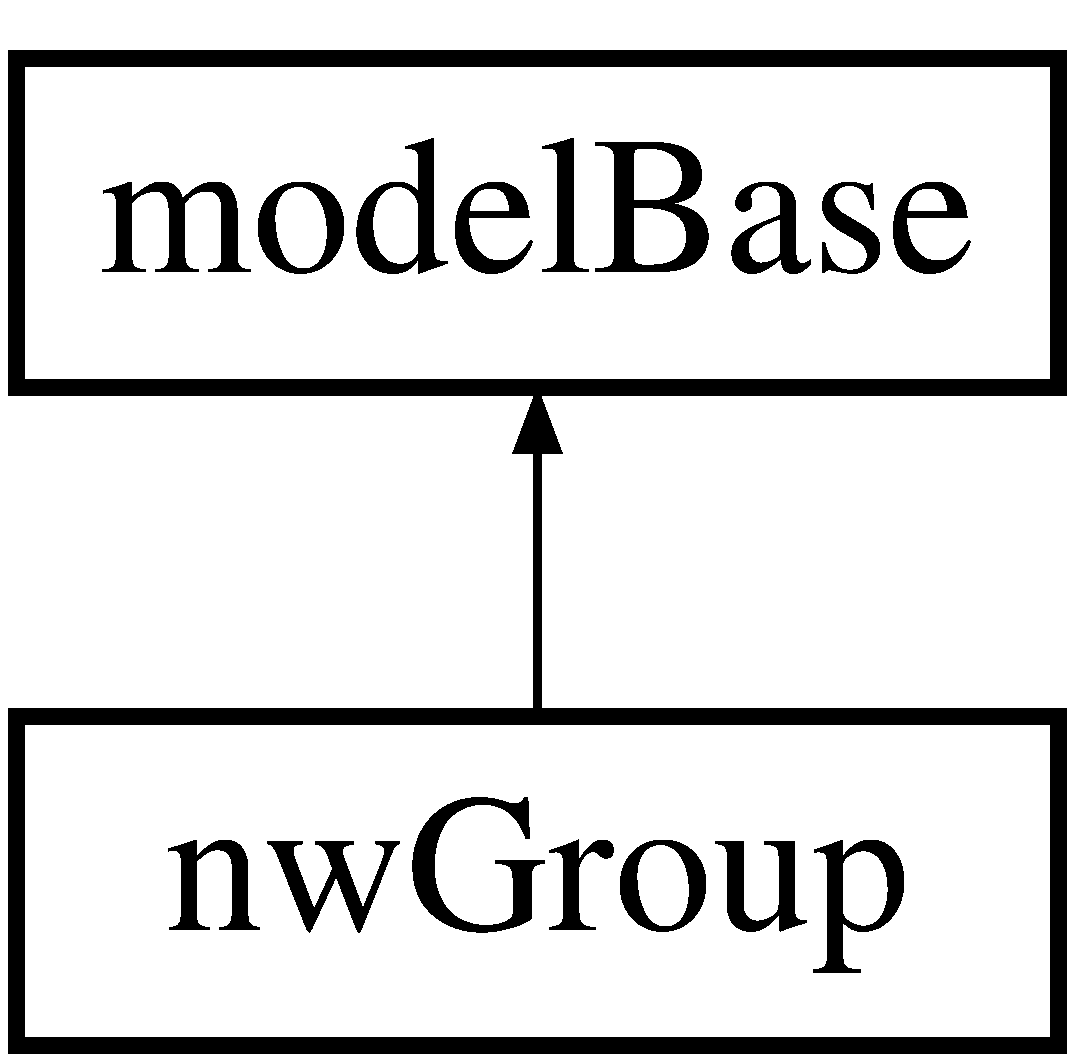
\includegraphics[height=2.000000cm]{classnwGroup}
\end{center}
\end{figure}


The documentation for this class was generated from the following file\-:\begin{DoxyCompactItemize}
\item 
engine/lib/builtins/auth/models.\-php\end{DoxyCompactItemize}

\hypertarget{classnwUser}{\section{nw\-User Class Reference}
\label{classnwUser}\index{nw\-User@{nw\-User}}
}
Inheritance diagram for nw\-User\-:\begin{figure}[H]
\begin{center}
\leavevmode
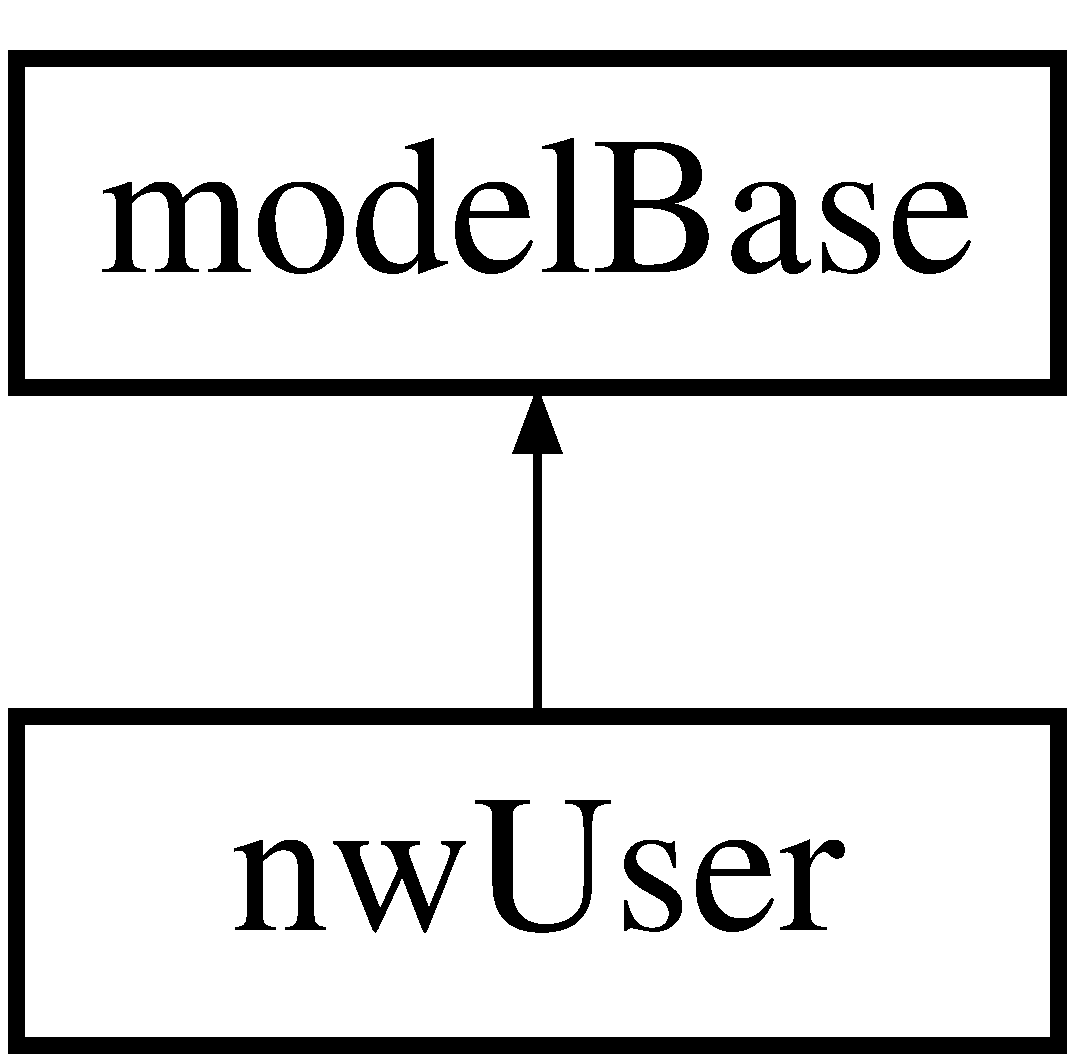
\includegraphics[height=2.000000cm]{classnwUser}
\end{center}
\end{figure}
\subsection*{Public Member Functions}
\begin{DoxyCompactItemize}
\item 
\hypertarget{classnwUser_a77d1c727701bbe971b1dfb8b8e0d7969}{{\bfseries set\-\_\-password} (\$newpass)}\label{classnwUser_a77d1c727701bbe971b1dfb8b8e0d7969}

\item 
\hypertarget{classnwUser_a72a9a2dff8b603498f59d4a29cf39547}{{\bfseries check\-\_\-password} (\$password)}\label{classnwUser_a72a9a2dff8b603498f59d4a29cf39547}

\item 
\hypertarget{classnwUser_a279737a0c576d840855c7d4249b0c904}{{\bfseries auth\-\_\-user} (\$pass)}\label{classnwUser_a279737a0c576d840855c7d4249b0c904}

\end{DoxyCompactItemize}


The documentation for this class was generated from the following file\-:\begin{DoxyCompactItemize}
\item 
engine/lib/builtins/auth/models.\-php\end{DoxyCompactItemize}

\hypertarget{classredirect}{\section{redirect Class Reference}
\label{classredirect}\index{redirect@{redirect}}
}
Inheritance diagram for redirect\-:\begin{figure}[H]
\begin{center}
\leavevmode
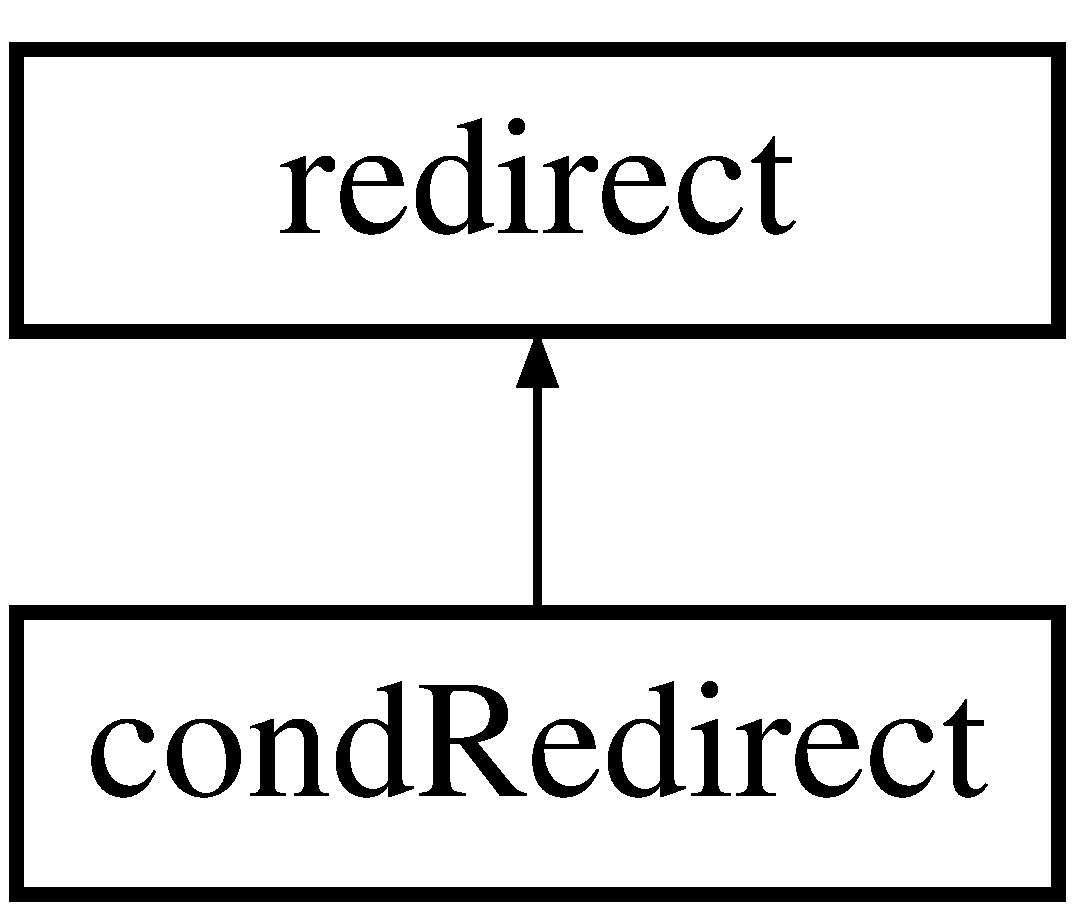
\includegraphics[height=2.000000cm]{classredirect}
\end{center}
\end{figure}
\subsection*{Public Member Functions}
\begin{DoxyCompactItemize}
\item 
\hyperlink{classredirect_aeb75fcecd20f097028211f5a56d929e7}{\-\_\-\-\_\-construct} (\$origin, \$destination)
\item 
\hyperlink{classredirect_a87c9d9aae382680b6e178229aaf56ce7}{view} (\$print=False)
\item 
\hyperlink{classredirect_a17326a08f9ee54def5ba1009a921b497}{to\-Html} (\$show\-Origin=false)
\item 
\hyperlink{classredirect_a7ebcebe7835af89c6b1a1f923a0721d9}{apply} (\$type)
\end{DoxyCompactItemize}
\subsection*{Public Attributes}
\begin{DoxyCompactItemize}
\item 
\hypertarget{classredirect_a30f64965b315e2710cd0376b5a57d214}{{\bfseries \$destination}}\label{classredirect_a30f64965b315e2710cd0376b5a57d214}

\end{DoxyCompactItemize}
\subsection*{Protected Attributes}
\begin{DoxyCompactItemize}
\item 
\hypertarget{classredirect_ad2813e1fba10299accc9939399a5e3ee}{{\bfseries \$origin}}\label{classredirect_ad2813e1fba10299accc9939399a5e3ee}

\end{DoxyCompactItemize}


\subsection{Detailed Description}
Provides a class for managing redirecting a page. The class accepts a destination and origin and allows for a redirect to be applied at any time, providing an advantage over using only P\-H\-P's builtin redirect resources.

\begin{DoxyAuthor}{Author}
Nate Levesque \href{mailto:public@thenaterhood.com}{\tt public@thenaterhood.\-com} Provides a class for storing and applying a redirect to another area of a website. 
\end{DoxyAuthor}


\subsection{Constructor \& Destructor Documentation}
\hypertarget{classredirect_aeb75fcecd20f097028211f5a56d929e7}{\index{redirect@{redirect}!\-\_\-\-\_\-construct@{\-\_\-\-\_\-construct}}
\index{\-\_\-\-\_\-construct@{\-\_\-\-\_\-construct}!redirect@{redirect}}
\subsubsection[{\-\_\-\-\_\-construct}]{\setlength{\rightskip}{0pt plus 5cm}redirect\-::\-\_\-\-\_\-construct (
\begin{DoxyParamCaption}
\item[{}]{\$origin, }
\item[{}]{\$destination}
\end{DoxyParamCaption}
)}}\label{classredirect_aeb75fcecd20f097028211f5a56d929e7}
Produces an instance of the class


\begin{DoxyParams}{Parameters}
{\em \$origin} & -\/ the url accessed originally \\
\hline
{\em \$destination} & -\/ the url to redirect to \\
\hline
\end{DoxyParams}


\subsection{Member Function Documentation}
\hypertarget{classredirect_a7ebcebe7835af89c6b1a1f923a0721d9}{\index{redirect@{redirect}!apply@{apply}}
\index{apply@{apply}!redirect@{redirect}}
\subsubsection[{apply}]{\setlength{\rightskip}{0pt plus 5cm}redirect\-::apply (
\begin{DoxyParamCaption}
\item[{}]{\$type}
\end{DoxyParamCaption}
)}}\label{classredirect_a7ebcebe7835af89c6b1a1f923a0721d9}
Applies the redirect to the page


\begin{DoxyParams}{Parameters}
{\em \$type} & -\/ the type of redirect to use \\
\hline
\end{DoxyParams}
\hypertarget{classredirect_a17326a08f9ee54def5ba1009a921b497}{\index{redirect@{redirect}!to\-Html@{to\-Html}}
\index{to\-Html@{to\-Html}!redirect@{redirect}}
\subsubsection[{to\-Html}]{\setlength{\rightskip}{0pt plus 5cm}redirect\-::to\-Html (
\begin{DoxyParamCaption}
\item[{}]{\$show\-Origin = {\ttfamily false}}
\end{DoxyParamCaption}
)}}\label{classredirect_a17326a08f9ee54def5ba1009a921b497}
Provides a simple text output to check if the class was initiated correctly \hypertarget{classredirect_a87c9d9aae382680b6e178229aaf56ce7}{\index{redirect@{redirect}!view@{view}}
\index{view@{view}!redirect@{redirect}}
\subsubsection[{view}]{\setlength{\rightskip}{0pt plus 5cm}redirect\-::view (
\begin{DoxyParamCaption}
\item[{}]{\$print = {\ttfamily False}}
\end{DoxyParamCaption}
)}}\label{classredirect_a87c9d9aae382680b6e178229aaf56ce7}
Provides a simple text output to check if the class was initiated correctly 

The documentation for this class was generated from the following file\-:\begin{DoxyCompactItemize}
\item 
engine/classes/class\-\_\-redirect.\-php\end{DoxyCompactItemize}

\hypertarget{classrequest}{\section{request Class Reference}
\label{classrequest}\index{request@{request}}
}
\subsection*{Static Public Member Functions}
\begin{DoxyCompactItemize}
\item 
static \hyperlink{classrequest_af5a8fd0735268d19657c87848b5827c4}{get\-\_\-sanitized} (\$varnames)
\item 
static \hyperlink{classrequest_abc216f18819cc535803c10177e6b89a6}{get\-\_\-sanitized\-\_\-as\-\_\-object} (\$varnames)
\item 
static \hyperlink{classrequest_a34d4adad12486829a5c14719a298797c}{sanitized\-\_\-get} (\$varname)
\item 
static \hyperlink{classrequest_a21f215aed587e3bfa86b3d2cf1f666f6}{sanitized\-\_\-post} (\$varname)
\item 
static \hyperlink{classrequest_a053c8d3b0c70d2d0f6db4810d9f0b3ba}{sanitized\-\_\-cookie} (\$varname)
\item 
static \hyperlink{classrequest_a37ee0eb6206a252716bc33cd4c0e7916}{default\-\_\-value} (\$varname)
\item 
static \hyperlink{classrequest_abac59171326160dc151ded6601f8da37}{meta} (\$varname)
\item 
static \hyperlink{classrequest_a544f6a832bdef9bd3857082da95887b6}{post} (\$varname)
\item 
static \hyperlink{classrequest_a322e929c6e065ccf688769109400b43b}{get} (\$varname)
\item 
static \hyperlink{classrequest_acb2ddb22763f6a73e2e5c4990edc277e}{cookie} (\$varname)
\item 
static \hyperlink{classrequest_aadbff81f737c00e5a9d634df19bc47cc}{sanitize} (\$dirty, \$maxlength=0)
\end{DoxyCompactItemize}


\subsection{Detailed Description}
Provides access and sanitation functions for retrieving data from P\-H\-P H\-T\-T\-P variables.

\begin{DoxyAuthor}{Author}
Nate Levesque \href{mailto:public@thenaterhood.com}{\tt public@thenaterhood.\-com} 
\end{DoxyAuthor}


\subsection{Member Function Documentation}
\hypertarget{classrequest_acb2ddb22763f6a73e2e5c4990edc277e}{\index{request@{request}!cookie@{cookie}}
\index{cookie@{cookie}!request@{request}}
\subsubsection[{cookie}]{\setlength{\rightskip}{0pt plus 5cm}static request\-::cookie (
\begin{DoxyParamCaption}
\item[{}]{\$varname}
\end{DoxyParamCaption}
)\hspace{0.3cm}{\ttfamily [static]}}}\label{classrequest_acb2ddb22763f6a73e2e5c4990edc277e}
Returns a raw value from the cookie array without sanitizing it, or an empty string if it doesn't exist. 
\begin{DoxyParams}[1]{Parameters}
type & {\em \$varname} & -\/ the name of the variable \\
\hline
\end{DoxyParams}
\begin{DoxyReturn}{Returns}
string -\/ the value of the variable 
\end{DoxyReturn}
\hypertarget{classrequest_a37ee0eb6206a252716bc33cd4c0e7916}{\index{request@{request}!default\-\_\-value@{default\-\_\-value}}
\index{default\-\_\-value@{default\-\_\-value}!request@{request}}
\subsubsection[{default\-\_\-value}]{\setlength{\rightskip}{0pt plus 5cm}static request\-::default\-\_\-value (
\begin{DoxyParamCaption}
\item[{}]{\$varname}
\end{DoxyParamCaption}
)\hspace{0.3cm}{\ttfamily [static]}}}\label{classrequest_a37ee0eb6206a252716bc33cd4c0e7916}
Returns the default value for a variable name as configured in the settings.\-php file.


\begin{DoxyParams}[1]{Parameters}
type & {\em \$varname} & -\/ the name of the variable \\
\hline
\end{DoxyParams}
\begin{DoxyReturn}{Returns}
type -\/ the default value 
\end{DoxyReturn}
\hypertarget{classrequest_a322e929c6e065ccf688769109400b43b}{\index{request@{request}!get@{get}}
\index{get@{get}!request@{request}}
\subsubsection[{get}]{\setlength{\rightskip}{0pt plus 5cm}static request\-::get (
\begin{DoxyParamCaption}
\item[{}]{\$varname}
\end{DoxyParamCaption}
)\hspace{0.3cm}{\ttfamily [static]}}}\label{classrequest_a322e929c6e065ccf688769109400b43b}
Returns a raw value from the G\-E\-T array without sanitizing it, or an empty string if it doesn't exist. 
\begin{DoxyParams}[1]{Parameters}
type & {\em \$varname} & -\/ the name of the variable \\
\hline
\end{DoxyParams}
\begin{DoxyReturn}{Returns}
string -\/ the value of the variable 
\end{DoxyReturn}
\hypertarget{classrequest_af5a8fd0735268d19657c87848b5827c4}{\index{request@{request}!get\-\_\-sanitized@{get\-\_\-sanitized}}
\index{get\-\_\-sanitized@{get\-\_\-sanitized}!request@{request}}
\subsubsection[{get\-\_\-sanitized}]{\setlength{\rightskip}{0pt plus 5cm}static request\-::get\-\_\-sanitized (
\begin{DoxyParamCaption}
\item[{}]{\$varnames}
\end{DoxyParamCaption}
)\hspace{0.3cm}{\ttfamily [static]}}}\label{classrequest_af5a8fd0735268d19657c87848b5827c4}
Returns an array of variables retrieved and sanitized from (in order of precedence) \$\-\_\-\-P\-O\-S\-T, \$\-\_\-\-G\-E\-T, \$\-\_\-\-C\-O\-O\-K\-I\-E and a default value if configured.


\begin{DoxyParams}[1]{Parameters}
type & {\em \$varnames} & -\/ an array of variable names \\
\hline
\end{DoxyParams}
\begin{DoxyReturn}{Returns}
type -\/ an array of cleaned variable values. 
\end{DoxyReturn}
\hypertarget{classrequest_abc216f18819cc535803c10177e6b89a6}{\index{request@{request}!get\-\_\-sanitized\-\_\-as\-\_\-object@{get\-\_\-sanitized\-\_\-as\-\_\-object}}
\index{get\-\_\-sanitized\-\_\-as\-\_\-object@{get\-\_\-sanitized\-\_\-as\-\_\-object}!request@{request}}
\subsubsection[{get\-\_\-sanitized\-\_\-as\-\_\-object}]{\setlength{\rightskip}{0pt plus 5cm}static request\-::get\-\_\-sanitized\-\_\-as\-\_\-object (
\begin{DoxyParamCaption}
\item[{}]{\$varnames}
\end{DoxyParamCaption}
)\hspace{0.3cm}{\ttfamily [static]}}}\label{classrequest_abc216f18819cc535803c10177e6b89a6}
Returns an object with the requested variables cleaned. This is primarily to take the place of the session class from previous versions. It acts as a drop-\/in replacement. Uses the get\-\_\-sanitized function internally then casts the array to an object.


\begin{DoxyParams}[1]{Parameters}
type & {\em \$varnames} & -\/ an array of variable names to find \\
\hline
\end{DoxyParams}
\begin{DoxyReturn}{Returns}
type -\/ an std\-Class instance containing the requested variables as fields. 
\end{DoxyReturn}
\hypertarget{classrequest_abac59171326160dc151ded6601f8da37}{\index{request@{request}!meta@{meta}}
\index{meta@{meta}!request@{request}}
\subsubsection[{meta}]{\setlength{\rightskip}{0pt plus 5cm}static request\-::meta (
\begin{DoxyParamCaption}
\item[{}]{\$varname}
\end{DoxyParamCaption}
)\hspace{0.3cm}{\ttfamily [static]}}}\label{classrequest_abac59171326160dc151ded6601f8da37}
Returns meta information from the S\-E\-R\-V\-E\-R array or an empty string if it doesn't exist.


\begin{DoxyParams}[1]{Parameters}
type & {\em \$varname} & -\/ the name of the variable \\
\hline
\end{DoxyParams}
\begin{DoxyReturn}{Returns}
string -\/ the value of the variable 
\end{DoxyReturn}
\hypertarget{classrequest_a544f6a832bdef9bd3857082da95887b6}{\index{request@{request}!post@{post}}
\index{post@{post}!request@{request}}
\subsubsection[{post}]{\setlength{\rightskip}{0pt plus 5cm}static request\-::post (
\begin{DoxyParamCaption}
\item[{}]{\$varname}
\end{DoxyParamCaption}
)\hspace{0.3cm}{\ttfamily [static]}}}\label{classrequest_a544f6a832bdef9bd3857082da95887b6}
Returns a raw value from the P\-O\-S\-T array without sanitizing it, or an empty string if it doesn't exist. 
\begin{DoxyParams}[1]{Parameters}
type & {\em \$varname} & -\/ the name of the variable \\
\hline
\end{DoxyParams}
\begin{DoxyReturn}{Returns}
string -\/ the value of the variable 
\end{DoxyReturn}
\hypertarget{classrequest_aadbff81f737c00e5a9d634df19bc47cc}{\index{request@{request}!sanitize@{sanitize}}
\index{sanitize@{sanitize}!request@{request}}
\subsubsection[{sanitize}]{\setlength{\rightskip}{0pt plus 5cm}static request\-::sanitize (
\begin{DoxyParamCaption}
\item[{}]{\$dirty, }
\item[{}]{\$maxlength = {\ttfamily 0}}
\end{DoxyParamCaption}
)\hspace{0.3cm}{\ttfamily [static]}}}\label{classrequest_aadbff81f737c00e5a9d634df19bc47cc}
Verify that a string is made of html-\/safe characters and short enough to fit where it belongs. Basically some simple input sanitizing for nonsecure things. \hypertarget{classrequest_a053c8d3b0c70d2d0f6db4810d9f0b3ba}{\index{request@{request}!sanitized\-\_\-cookie@{sanitized\-\_\-cookie}}
\index{sanitized\-\_\-cookie@{sanitized\-\_\-cookie}!request@{request}}
\subsubsection[{sanitized\-\_\-cookie}]{\setlength{\rightskip}{0pt plus 5cm}static request\-::sanitized\-\_\-cookie (
\begin{DoxyParamCaption}
\item[{}]{\$varname}
\end{DoxyParamCaption}
)\hspace{0.3cm}{\ttfamily [static]}}}\label{classrequest_a053c8d3b0c70d2d0f6db4810d9f0b3ba}
Returns a sanitized variable value from the cookie array or an empty string if it doesn't exist.


\begin{DoxyParams}[1]{Parameters}
type & {\em \$varname} & -\/ the name of the variable \\
\hline
\end{DoxyParams}
\begin{DoxyReturn}{Returns}
string -\/ the value of the variable 
\end{DoxyReturn}
\hypertarget{classrequest_a34d4adad12486829a5c14719a298797c}{\index{request@{request}!sanitized\-\_\-get@{sanitized\-\_\-get}}
\index{sanitized\-\_\-get@{sanitized\-\_\-get}!request@{request}}
\subsubsection[{sanitized\-\_\-get}]{\setlength{\rightskip}{0pt plus 5cm}static request\-::sanitized\-\_\-get (
\begin{DoxyParamCaption}
\item[{}]{\$varname}
\end{DoxyParamCaption}
)\hspace{0.3cm}{\ttfamily [static]}}}\label{classrequest_a34d4adad12486829a5c14719a298797c}
Returns a sanitized variable value from the get array or an empty string if it doesn't exist.


\begin{DoxyParams}[1]{Parameters}
type & {\em \$varname} & -\/ the name of the variable \\
\hline
\end{DoxyParams}
\begin{DoxyReturn}{Returns}
string -\/ the value of the variable 
\end{DoxyReturn}
\hypertarget{classrequest_a21f215aed587e3bfa86b3d2cf1f666f6}{\index{request@{request}!sanitized\-\_\-post@{sanitized\-\_\-post}}
\index{sanitized\-\_\-post@{sanitized\-\_\-post}!request@{request}}
\subsubsection[{sanitized\-\_\-post}]{\setlength{\rightskip}{0pt plus 5cm}static request\-::sanitized\-\_\-post (
\begin{DoxyParamCaption}
\item[{}]{\$varname}
\end{DoxyParamCaption}
)\hspace{0.3cm}{\ttfamily [static]}}}\label{classrequest_a21f215aed587e3bfa86b3d2cf1f666f6}
Returns a sanitized variable value from the post array or an empty string if it doesn't exist.


\begin{DoxyParams}[1]{Parameters}
type & {\em \$varname} & -\/ the name of the variable \\
\hline
\end{DoxyParams}
\begin{DoxyReturn}{Returns}
string -\/ the value of the variable 
\end{DoxyReturn}


The documentation for this class was generated from the following file\-:\begin{DoxyCompactItemize}
\item 
engine/classes/class\-\_\-request.\-php\end{DoxyCompactItemize}

\hypertarget{classSessionMgr}{\section{Session\-Mgr Class Reference}
\label{classSessionMgr}\index{Session\-Mgr@{Session\-Mgr}}
}
\subsection*{Public Member Functions}
\begin{DoxyCompactItemize}
\item 
\hyperlink{classSessionMgr_aedbc4cb2228951b67f6176c95a9c177a}{get\-\_\-csrf\-\_\-id} ()
\item 
\hyperlink{classSessionMgr_a6fc75c805601b86bf75e32e74a5dec16}{get\-\_\-csrf\-\_\-token} ()
\item 
\hyperlink{classSessionMgr_ac1a7c2c9873c8f7b64aef607ab96bc78}{check\-\_\-csrf} (\$method)
\item 
\hyperlink{classSessionMgr_aafc03db5cc80b14a459c81a99865b91b}{form\-\_\-names} (\$names, \$regenerate)
\item 
\hyperlink{classSessionMgr_a54067567a91677f592751bcc3096b175}{start\-Session} ()
\item 
\hyperlink{classSessionMgr_a65a1ebe7f9d219bdb88efa18df697295}{\-\_\-\-\_\-set} (\$name, \$value)
\item 
\hyperlink{classSessionMgr_a0c2ca3fa3663059b2490c80897f8d437}{\-\_\-\-\_\-get} (\$name)
\item 
\hypertarget{classSessionMgr_a992329fbe672857d8fd74ebee57329bc}{{\bfseries \-\_\-\-\_\-isset} (\$name)}\label{classSessionMgr_a992329fbe672857d8fd74ebee57329bc}

\item 
\hypertarget{classSessionMgr_ac3cec7da4442db2d333f1ca0a693e1e0}{{\bfseries \-\_\-\-\_\-unset} (\$name)}\label{classSessionMgr_ac3cec7da4442db2d333f1ca0a693e1e0}

\item 
\hypertarget{classSessionMgr_a5eecf3a633697c6dbcd6052575629423}{{\bfseries destroy} ()}\label{classSessionMgr_a5eecf3a633697c6dbcd6052575629423}

\end{DoxyCompactItemize}
\subsection*{Static Public Member Functions}
\begin{DoxyCompactItemize}
\item 
static \hyperlink{classSessionMgr_a089318cf1224b6c02cc755aee63a1d9c}{get\-Instance} ()
\end{DoxyCompactItemize}
\subsection*{Public Attributes}
\begin{DoxyCompactItemize}
\item 
\hypertarget{classSessionMgr_aa3b423ebb39b16714c0baec2d2a6df8d}{const {\bfseries S\-E\-S\-S\-I\-O\-N\-\_\-\-S\-T\-A\-R\-T\-E\-D} = True}\label{classSessionMgr_aa3b423ebb39b16714c0baec2d2a6df8d}

\item 
\hypertarget{classSessionMgr_acc8882dff09da4854e1b02245f25de95}{const {\bfseries S\-E\-S\-S\-I\-O\-N\-\_\-\-N\-O\-T\-\_\-\-S\-T\-A\-R\-T\-E\-D} = False}\label{classSessionMgr_acc8882dff09da4854e1b02245f25de95}

\end{DoxyCompactItemize}


\subsection{Member Function Documentation}
\hypertarget{classSessionMgr_a0c2ca3fa3663059b2490c80897f8d437}{\index{Session\-Mgr@{Session\-Mgr}!\-\_\-\-\_\-get@{\-\_\-\-\_\-get}}
\index{\-\_\-\-\_\-get@{\-\_\-\-\_\-get}!SessionMgr@{Session\-Mgr}}
\subsubsection[{\-\_\-\-\_\-get}]{\setlength{\rightskip}{0pt plus 5cm}Session\-Mgr\-::\-\_\-\-\_\-get (
\begin{DoxyParamCaption}
\item[{}]{\$name}
\end{DoxyParamCaption}
)}}\label{classSessionMgr_a0c2ca3fa3663059b2490c80897f8d437}
Retrieves data from the session \hypertarget{classSessionMgr_a65a1ebe7f9d219bdb88efa18df697295}{\index{Session\-Mgr@{Session\-Mgr}!\-\_\-\-\_\-set@{\-\_\-\-\_\-set}}
\index{\-\_\-\-\_\-set@{\-\_\-\-\_\-set}!SessionMgr@{Session\-Mgr}}
\subsubsection[{\-\_\-\-\_\-set}]{\setlength{\rightskip}{0pt plus 5cm}Session\-Mgr\-::\-\_\-\-\_\-set (
\begin{DoxyParamCaption}
\item[{}]{\$name, }
\item[{}]{\$value}
\end{DoxyParamCaption}
)}}\label{classSessionMgr_a65a1ebe7f9d219bdb88efa18df697295}
Allows for storing data into the session \hypertarget{classSessionMgr_ac1a7c2c9873c8f7b64aef607ab96bc78}{\index{Session\-Mgr@{Session\-Mgr}!check\-\_\-csrf@{check\-\_\-csrf}}
\index{check\-\_\-csrf@{check\-\_\-csrf}!SessionMgr@{Session\-Mgr}}
\subsubsection[{check\-\_\-csrf}]{\setlength{\rightskip}{0pt plus 5cm}Session\-Mgr\-::check\-\_\-csrf (
\begin{DoxyParamCaption}
\item[{}]{\$method}
\end{DoxyParamCaption}
)}}\label{classSessionMgr_ac1a7c2c9873c8f7b64aef607ab96bc78}
Checks the validity of the C\-S\-R\-F token from the given method (post or get) \hypertarget{classSessionMgr_aafc03db5cc80b14a459c81a99865b91b}{\index{Session\-Mgr@{Session\-Mgr}!form\-\_\-names@{form\-\_\-names}}
\index{form\-\_\-names@{form\-\_\-names}!SessionMgr@{Session\-Mgr}}
\subsubsection[{form\-\_\-names}]{\setlength{\rightskip}{0pt plus 5cm}Session\-Mgr\-::form\-\_\-names (
\begin{DoxyParamCaption}
\item[{}]{\$names, }
\item[{}]{\$regenerate}
\end{DoxyParamCaption}
)}}\label{classSessionMgr_aafc03db5cc80b14a459c81a99865b91b}
Generates csrf-\/safe form names for a form. \hypertarget{classSessionMgr_aedbc4cb2228951b67f6176c95a9c177a}{\index{Session\-Mgr@{Session\-Mgr}!get\-\_\-csrf\-\_\-id@{get\-\_\-csrf\-\_\-id}}
\index{get\-\_\-csrf\-\_\-id@{get\-\_\-csrf\-\_\-id}!SessionMgr@{Session\-Mgr}}
\subsubsection[{get\-\_\-csrf\-\_\-id}]{\setlength{\rightskip}{0pt plus 5cm}Session\-Mgr\-::get\-\_\-csrf\-\_\-id (
\begin{DoxyParamCaption}
{}
\end{DoxyParamCaption}
)}}\label{classSessionMgr_aedbc4cb2228951b67f6176c95a9c177a}
Returns the csrf token id \hypertarget{classSessionMgr_a6fc75c805601b86bf75e32e74a5dec16}{\index{Session\-Mgr@{Session\-Mgr}!get\-\_\-csrf\-\_\-token@{get\-\_\-csrf\-\_\-token}}
\index{get\-\_\-csrf\-\_\-token@{get\-\_\-csrf\-\_\-token}!SessionMgr@{Session\-Mgr}}
\subsubsection[{get\-\_\-csrf\-\_\-token}]{\setlength{\rightskip}{0pt plus 5cm}Session\-Mgr\-::get\-\_\-csrf\-\_\-token (
\begin{DoxyParamCaption}
{}
\end{DoxyParamCaption}
)}}\label{classSessionMgr_a6fc75c805601b86bf75e32e74a5dec16}
Returns the value of the C\-S\-R\-F token \hypertarget{classSessionMgr_a089318cf1224b6c02cc755aee63a1d9c}{\index{Session\-Mgr@{Session\-Mgr}!get\-Instance@{get\-Instance}}
\index{get\-Instance@{get\-Instance}!SessionMgr@{Session\-Mgr}}
\subsubsection[{get\-Instance}]{\setlength{\rightskip}{0pt plus 5cm}static Session\-Mgr\-::get\-Instance (
\begin{DoxyParamCaption}
{}
\end{DoxyParamCaption}
)\hspace{0.3cm}{\ttfamily [static]}}}\label{classSessionMgr_a089318cf1224b6c02cc755aee63a1d9c}
Returns the instance of the session and automatically initializes it if necessary \hypertarget{classSessionMgr_a54067567a91677f592751bcc3096b175}{\index{Session\-Mgr@{Session\-Mgr}!start\-Session@{start\-Session}}
\index{start\-Session@{start\-Session}!SessionMgr@{Session\-Mgr}}
\subsubsection[{start\-Session}]{\setlength{\rightskip}{0pt plus 5cm}Session\-Mgr\-::start\-Session (
\begin{DoxyParamCaption}
{}
\end{DoxyParamCaption}
)}}\label{classSessionMgr_a54067567a91677f592751bcc3096b175}
Starts or restarts the session 

The documentation for this class was generated from the following file\-:\begin{DoxyCompactItemize}
\item 
engine/classes/class\-\_\-session\-Mgr.\-php\end{DoxyCompactItemize}

\hypertarget{classsitemaps}{\section{sitemaps Class Reference}
\label{classsitemaps}\index{sitemaps@{sitemaps}}
}
Inheritance diagram for sitemaps\-:\begin{figure}[H]
\begin{center}
\leavevmode
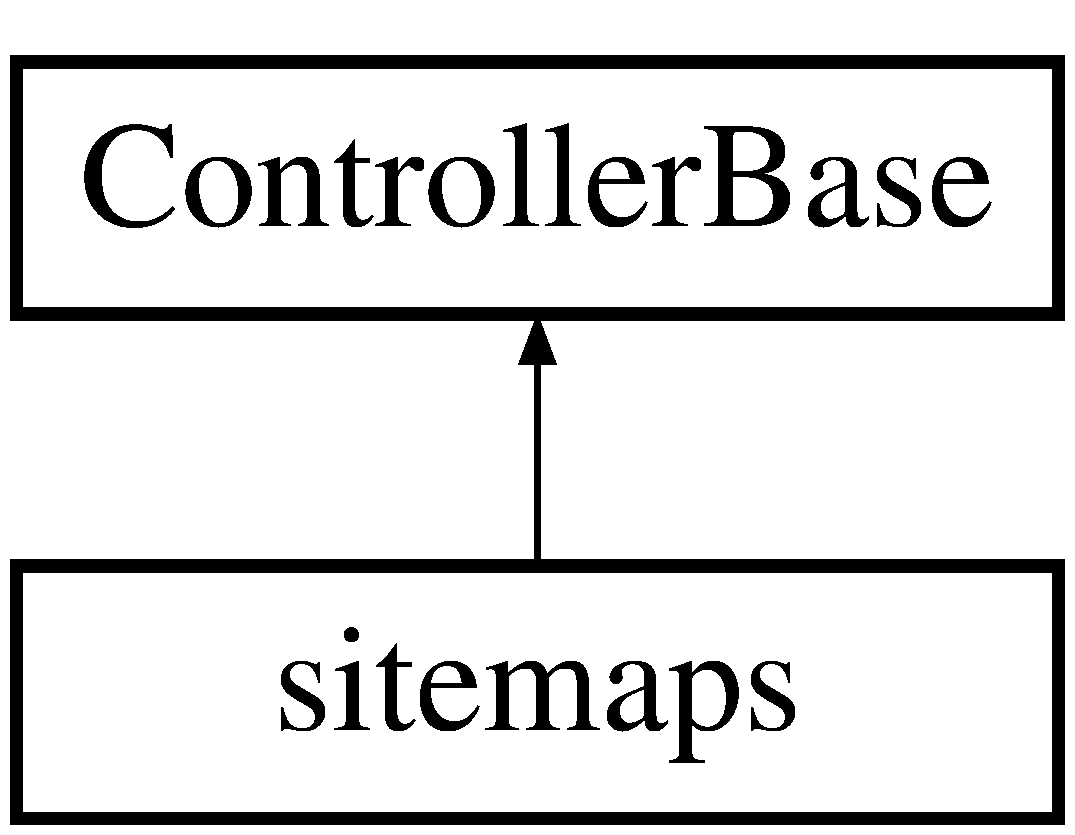
\includegraphics[height=2.000000cm]{classsitemaps}
\end{center}
\end{figure}
\subsection*{Public Member Functions}
\begin{DoxyCompactItemize}
\item 
\hypertarget{classsitemaps_a8b19067e6e0027d49a8d7ddfedec5cbd}{{\bfseries \-\_\-\-\_\-call} (\$method, \$args)}\label{classsitemaps_a8b19067e6e0027d49a8d7ddfedec5cbd}

\end{DoxyCompactItemize}
\subsection*{Additional Inherited Members}


The documentation for this class was generated from the following file\-:\begin{DoxyCompactItemize}
\item 
engine/lib/builtins/sitemaps/main.\-php\end{DoxyCompactItemize}

\hypertarget{classstdClassArticle}{\section{std\-Class\-Article Class Reference}
\label{classstdClassArticle}\index{std\-Class\-Article@{std\-Class\-Article}}
}
Inheritance diagram for std\-Class\-Article\-:\begin{figure}[H]
\begin{center}
\leavevmode
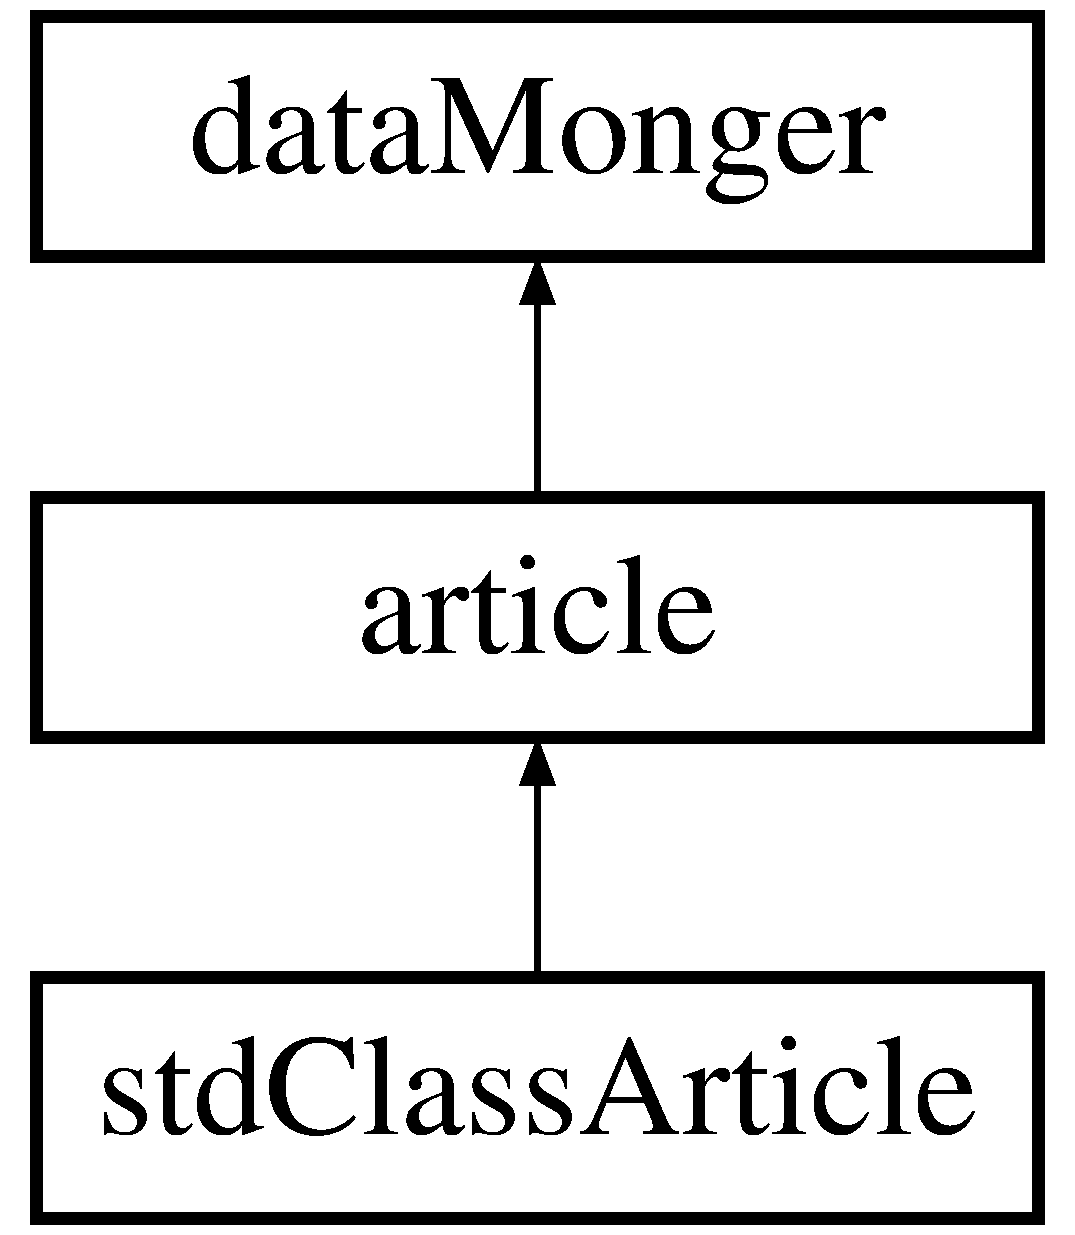
\includegraphics[height=3.000000cm]{classstdClassArticle}
\end{center}
\end{figure}
\subsection*{Public Member Functions}
\begin{DoxyCompactItemize}
\item 
\hypertarget{classstdClassArticle_aa8cf609eced5a90e21928f3cdc230ac3}{{\bfseries \-\_\-\-\_\-construct} (\$std\-Class)}\label{classstdClassArticle_aa8cf609eced5a90e21928f3cdc230ac3}

\end{DoxyCompactItemize}
\subsection*{Additional Inherited Members}


The documentation for this class was generated from the following file\-:\begin{DoxyCompactItemize}
\item 
engine/classes/class\-\_\-std\-Class\-Article.\-php\end{DoxyCompactItemize}

\hypertarget{classurl}{\section{url Class Reference}
\label{classurl}\index{url@{url}}
}
Inheritance diagram for url\-:\begin{figure}[H]
\begin{center}
\leavevmode
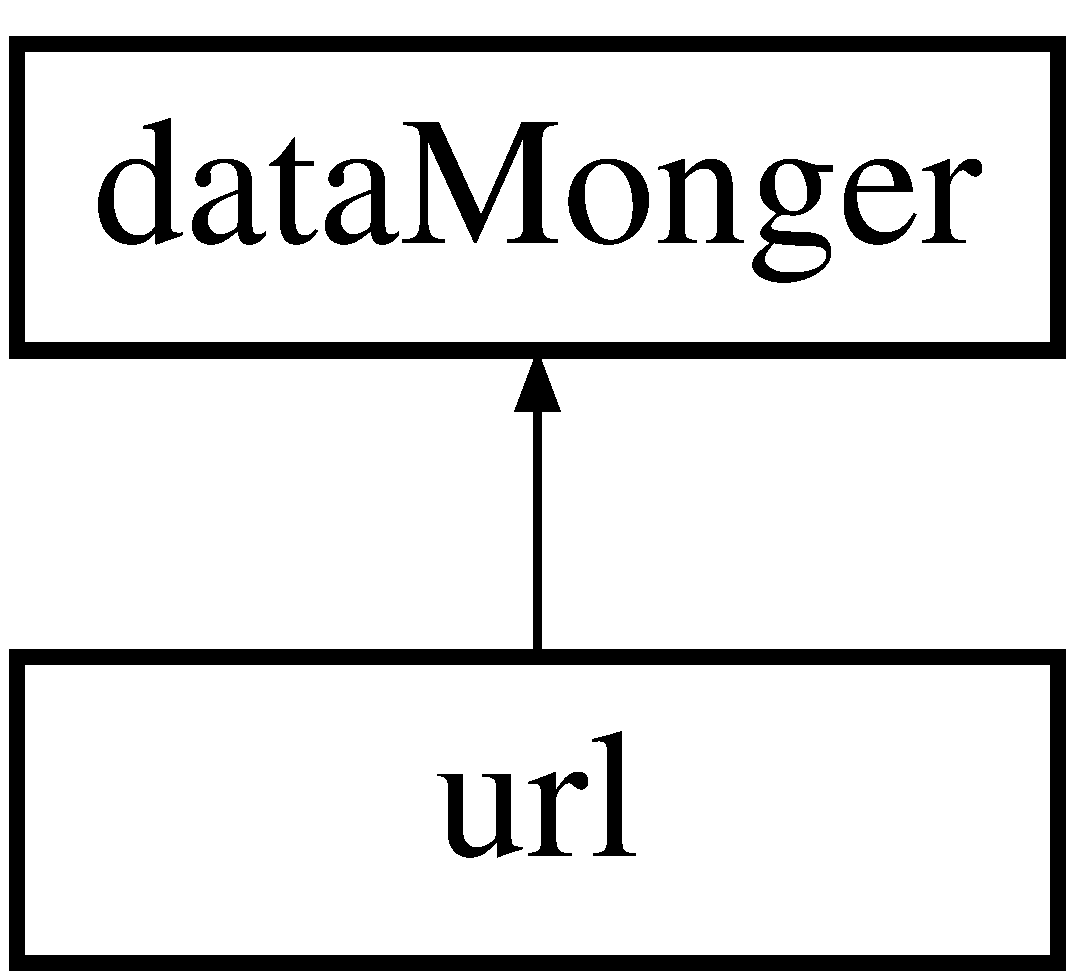
\includegraphics[height=2.000000cm]{classurl}
\end{center}
\end{figure}
\subsection*{Public Member Functions}
\begin{DoxyCompactItemize}
\item 
\hyperlink{classurl_a5c24c6c8c78702fd4481a164dda74a00}{\-\_\-\-\_\-construct} (\$link, \$lastmod)
\item 
\hyperlink{classurl_a5dc2bb0c65043a10c3f8489fbeeed1c6}{output} (\$type='Xml')
\item 
\hyperlink{classurl_a26bdef3d54b526a2bcb27dd7b89b1a1d}{to\-Xml} ()
\item 
\hypertarget{classurl_af1c2d232c6da6b3c3db4c09869d1a646}{{\bfseries to\-Html} ()}\label{classurl_af1c2d232c6da6b3c3db4c09869d1a646}

\end{DoxyCompactItemize}
\subsection*{Additional Inherited Members}


\subsection{Detailed Description}
Provides a resource for storing a representation of a page on a website with the location and modification date with the facilities to return it in xml format. Mainly for use in a sitemap. Includes the inherited class Represents a url object to store a sitemap url block 

\subsection{Constructor \& Destructor Documentation}
\hypertarget{classurl_a5c24c6c8c78702fd4481a164dda74a00}{\index{url@{url}!\-\_\-\-\_\-construct@{\-\_\-\-\_\-construct}}
\index{\-\_\-\-\_\-construct@{\-\_\-\-\_\-construct}!url@{url}}
\subsubsection[{\-\_\-\-\_\-construct}]{\setlength{\rightskip}{0pt plus 5cm}url\-::\-\_\-\-\_\-construct (
\begin{DoxyParamCaption}
\item[{}]{\$link, }
\item[{}]{\$lastmod}
\end{DoxyParamCaption}
)}}\label{classurl_a5c24c6c8c78702fd4481a164dda74a00}
Creates the data object to contain the atom feed item.


\begin{DoxyParams}{Parameters}
{\em \$link} & (str)\-: the web address of the item source \\
\hline
{\em \$lastmod} & (str)\-: the item modification date \\
\hline
\end{DoxyParams}


\subsection{Member Function Documentation}
\hypertarget{classurl_a5dc2bb0c65043a10c3f8489fbeeed1c6}{\index{url@{url}!output@{output}}
\index{output@{output}!url@{url}}
\subsubsection[{output}]{\setlength{\rightskip}{0pt plus 5cm}url\-::output (
\begin{DoxyParamCaption}
\item[{}]{\$type = {\ttfamily 'Xml'}}
\end{DoxyParamCaption}
)}}\label{classurl_a5dc2bb0c65043a10c3f8489fbeeed1c6}
Produces output in the requested format, defaulting to xml 
\begin{DoxyParams}{Parameters}
{\em \$output} & -\/ ignored \\
\hline
\end{DoxyParams}
\hypertarget{classurl_a26bdef3d54b526a2bcb27dd7b89b1a1d}{\index{url@{url}!to\-Xml@{to\-Xml}}
\index{to\-Xml@{to\-Xml}!url@{url}}
\subsubsection[{to\-Xml}]{\setlength{\rightskip}{0pt plus 5cm}url\-::to\-Xml (
\begin{DoxyParamCaption}
{}
\end{DoxyParamCaption}
)}}\label{classurl_a26bdef3d54b526a2bcb27dd7b89b1a1d}
Produces the coded output of the item that can be returned and displayed or saved

\begin{DoxyReturn}{Returns}
\$item -\/ an xml-\/encoded representation of the item 
\end{DoxyReturn}


The documentation for this class was generated from the following file\-:\begin{DoxyCompactItemize}
\item 
engine/classes/class\-\_\-url.\-php\end{DoxyCompactItemize}

\hypertarget{classurlHandler}{\section{url\-Handler Class Reference}
\label{classurlHandler}\index{url\-Handler@{url\-Handler}}
}
\subsection*{Public Member Functions}
\begin{DoxyCompactItemize}
\item 
\hyperlink{classurlHandler_ae4fbc10799a30bfed0adfb7e1bc4d065}{reparse\-Url} ()
\item 
\hyperlink{classurlHandler_ac15274538beabbd91be8806e34a8d0a5}{get\-Controller} ()
\item 
\hyperlink{classurlHandler_a7791427f40a3a6bd741d03eb0273ebf0}{get\-Controller\-Id} ()
\end{DoxyCompactItemize}


\subsection{Detailed Description}
Contains functionality for handling and routing U\-R\-Ls

\begin{DoxyAuthor}{Author}
Nate Levesque \href{mailto:public@thenaterhood.com}{\tt public@thenaterhood.\-com} Include the main blog functionality A class for managing U\-R\-L related data 
\end{DoxyAuthor}


\subsection{Member Function Documentation}
\hypertarget{classurlHandler_ac15274538beabbd91be8806e34a8d0a5}{\index{url\-Handler@{url\-Handler}!get\-Controller@{get\-Controller}}
\index{get\-Controller@{get\-Controller}!urlHandler@{url\-Handler}}
\subsubsection[{get\-Controller}]{\setlength{\rightskip}{0pt plus 5cm}url\-Handler\-::get\-Controller (
\begin{DoxyParamCaption}
{}
\end{DoxyParamCaption}
)}}\label{classurlHandler_ac15274538beabbd91be8806e34a8d0a5}
Returns the selected controller \begin{DoxyReturn}{Returns}
the name of the controller file 
\end{DoxyReturn}
\hypertarget{classurlHandler_a7791427f40a3a6bd741d03eb0273ebf0}{\index{url\-Handler@{url\-Handler}!get\-Controller\-Id@{get\-Controller\-Id}}
\index{get\-Controller\-Id@{get\-Controller\-Id}!urlHandler@{url\-Handler}}
\subsubsection[{get\-Controller\-Id}]{\setlength{\rightskip}{0pt plus 5cm}url\-Handler\-::get\-Controller\-Id (
\begin{DoxyParamCaption}
{}
\end{DoxyParamCaption}
)}}\label{classurlHandler_a7791427f40a3a6bd741d03eb0273ebf0}
Returns the controller I\-D \begin{DoxyReturn}{Returns}
the name of the controller 
\end{DoxyReturn}
\hypertarget{classurlHandler_ae4fbc10799a30bfed0adfb7e1bc4d065}{\index{url\-Handler@{url\-Handler}!reparse\-Url@{reparse\-Url}}
\index{reparse\-Url@{reparse\-Url}!urlHandler@{url\-Handler}}
\subsubsection[{reparse\-Url}]{\setlength{\rightskip}{0pt plus 5cm}url\-Handler\-::reparse\-Url (
\begin{DoxyParamCaption}
{}
\end{DoxyParamCaption}
)}}\label{classurlHandler_ae4fbc10799a30bfed0adfb7e1bc4d065}
Reparses the stored url data after removing the first element from it 

The documentation for this class was generated from the following file\-:\begin{DoxyCompactItemize}
\item 
engine/classes/class\-\_\-url\-Handler.\-php\end{DoxyCompactItemize}

\hypertarget{classurlset}{\section{urlset Class Reference}
\label{classurlset}\index{urlset@{urlset}}
}
\subsection*{Public Member Functions}
\begin{DoxyCompactItemize}
\item 
\hyperlink{classurlset_ac6c6925c7d52e398c7f1a348c32f9187}{\-\_\-\-\_\-construct} ()
\item 
\hyperlink{classurlset_a6d8beb22e64a52dd84e44c42424bf16a}{new\-\_\-item} (\$loc, \$lastmod)
\item 
\hyperlink{classurlset_a6e17ff78d5019fde200589415759e596}{to\-Xml} ()
\item 
\hypertarget{classurlset_a54d11e072a592f19fc8341b95407e2bc}{{\bfseries to\-Html} ()}\label{classurlset_a54d11e072a592f19fc8341b95407e2bc}

\end{DoxyCompactItemize}


\subsection{Detailed Description}
Provides a class for creating and containing a sitemap with the ability to export it as xml data. \begin{DoxyAuthor}{Author}
Nate Levesque \href{mailto:public@thenaterhood.com}{\tt public@thenaterhood.\-com} Include the required url class to use internally Defines a data object to contain an xml sitemap. 
\end{DoxyAuthor}


\subsection{Constructor \& Destructor Documentation}
\hypertarget{classurlset_ac6c6925c7d52e398c7f1a348c32f9187}{\index{urlset@{urlset}!\-\_\-\-\_\-construct@{\-\_\-\-\_\-construct}}
\index{\-\_\-\-\_\-construct@{\-\_\-\-\_\-construct}!urlset@{urlset}}
\subsubsection[{\-\_\-\-\_\-construct}]{\setlength{\rightskip}{0pt plus 5cm}urlset\-::\-\_\-\-\_\-construct (
\begin{DoxyParamCaption}
{}
\end{DoxyParamCaption}
)}}\label{classurlset_ac6c6925c7d52e398c7f1a348c32f9187}
Creates an empty sitemap class 

\subsection{Member Function Documentation}
\hypertarget{classurlset_a6d8beb22e64a52dd84e44c42424bf16a}{\index{urlset@{urlset}!new\-\_\-item@{new\-\_\-item}}
\index{new\-\_\-item@{new\-\_\-item}!urlset@{urlset}}
\subsubsection[{new\-\_\-item}]{\setlength{\rightskip}{0pt plus 5cm}urlset\-::new\-\_\-item (
\begin{DoxyParamCaption}
\item[{}]{\$loc, }
\item[{}]{\$lastmod}
\end{DoxyParamCaption}
)}}\label{classurlset_a6d8beb22e64a52dd84e44c42424bf16a}
Adds an item to the feed as an object in the object's items array


\begin{DoxyParams}{Parameters}
{\em \$loc} & (str)\-: the web address of the item's source \\
\hline
{\em \$lastmod} & (str)\-: the modification date of the item \\
\hline
\end{DoxyParams}
\hypertarget{classurlset_a6e17ff78d5019fde200589415759e596}{\index{urlset@{urlset}!to\-Xml@{to\-Xml}}
\index{to\-Xml@{to\-Xml}!urlset@{urlset}}
\subsubsection[{to\-Xml}]{\setlength{\rightskip}{0pt plus 5cm}urlset\-::to\-Xml (
\begin{DoxyParamCaption}
{}
\end{DoxyParamCaption}
)}}\label{classurlset_a6e17ff78d5019fde200589415759e596}
Returns a displayable representation of the sitemap with appropriate code added.

\begin{DoxyReturn}{Returns}
\$r (string) -\/ an xml encoded output of the class 
\end{DoxyReturn}


The documentation for this class was generated from the following file\-:\begin{DoxyCompactItemize}
\item 
engine/classes/class\-\_\-urlset.\-php\end{DoxyCompactItemize}

%--- End generated contents ---

% Index
\newpage
\phantomsection
\addcontentsline{toc}{chapter}{Index}
\printindex

\end{document}
